% Options for packages loaded elsewhere
\PassOptionsToPackage{unicode}{hyperref}
\PassOptionsToPackage{hyphens}{url}
\documentclass[
  12pt,
]{article}
\usepackage{xcolor}
\usepackage[margin=1in]{geometry}
\usepackage{amsmath,amssymb}
\setcounter{secnumdepth}{-\maxdimen} % remove section numbering
\usepackage{iftex}
\ifPDFTeX
  \usepackage[T1]{fontenc}
  \usepackage[utf8]{inputenc}
  \usepackage{textcomp} % provide euro and other symbols
\else % if luatex or xetex
  \usepackage{unicode-math} % this also loads fontspec
  \defaultfontfeatures{Scale=MatchLowercase}
  \defaultfontfeatures[\rmfamily]{Ligatures=TeX,Scale=1}
\fi
\usepackage{lmodern}
\ifPDFTeX\else
  % xetex/luatex font selection
\fi
% Use upquote if available, for straight quotes in verbatim environments
\IfFileExists{upquote.sty}{\usepackage{upquote}}{}
\IfFileExists{microtype.sty}{% use microtype if available
  \usepackage[]{microtype}
  \UseMicrotypeSet[protrusion]{basicmath} % disable protrusion for tt fonts
}{}
\usepackage{setspace}
\usepackage{color}
\usepackage{fancyvrb}
\newcommand{\VerbBar}{|}
\newcommand{\VERB}{\Verb[commandchars=\\\{\}]}
\DefineVerbatimEnvironment{Highlighting}{Verbatim}{commandchars=\\\{\}}
% Add ',fontsize=\small' for more characters per line
\newenvironment{Shaded}{}{}
\newcommand{\AlertTok}[1]{\textcolor[rgb]{1.00,0.00,0.00}{\textbf{#1}}}
\newcommand{\AnnotationTok}[1]{\textcolor[rgb]{0.38,0.63,0.69}{\textbf{\textit{#1}}}}
\newcommand{\AttributeTok}[1]{\textcolor[rgb]{0.49,0.56,0.16}{#1}}
\newcommand{\BaseNTok}[1]{\textcolor[rgb]{0.25,0.63,0.44}{#1}}
\newcommand{\BuiltInTok}[1]{\textcolor[rgb]{0.00,0.50,0.00}{#1}}
\newcommand{\CharTok}[1]{\textcolor[rgb]{0.25,0.44,0.63}{#1}}
\newcommand{\CommentTok}[1]{\textcolor[rgb]{0.38,0.63,0.69}{\textit{#1}}}
\newcommand{\CommentVarTok}[1]{\textcolor[rgb]{0.38,0.63,0.69}{\textbf{\textit{#1}}}}
\newcommand{\ConstantTok}[1]{\textcolor[rgb]{0.53,0.00,0.00}{#1}}
\newcommand{\ControlFlowTok}[1]{\textcolor[rgb]{0.00,0.44,0.13}{\textbf{#1}}}
\newcommand{\DataTypeTok}[1]{\textcolor[rgb]{0.56,0.13,0.00}{#1}}
\newcommand{\DecValTok}[1]{\textcolor[rgb]{0.25,0.63,0.44}{#1}}
\newcommand{\DocumentationTok}[1]{\textcolor[rgb]{0.73,0.13,0.13}{\textit{#1}}}
\newcommand{\ErrorTok}[1]{\textcolor[rgb]{1.00,0.00,0.00}{\textbf{#1}}}
\newcommand{\ExtensionTok}[1]{#1}
\newcommand{\FloatTok}[1]{\textcolor[rgb]{0.25,0.63,0.44}{#1}}
\newcommand{\FunctionTok}[1]{\textcolor[rgb]{0.02,0.16,0.49}{#1}}
\newcommand{\ImportTok}[1]{\textcolor[rgb]{0.00,0.50,0.00}{\textbf{#1}}}
\newcommand{\InformationTok}[1]{\textcolor[rgb]{0.38,0.63,0.69}{\textbf{\textit{#1}}}}
\newcommand{\KeywordTok}[1]{\textcolor[rgb]{0.00,0.44,0.13}{\textbf{#1}}}
\newcommand{\NormalTok}[1]{#1}
\newcommand{\OperatorTok}[1]{\textcolor[rgb]{0.40,0.40,0.40}{#1}}
\newcommand{\OtherTok}[1]{\textcolor[rgb]{0.00,0.44,0.13}{#1}}
\newcommand{\PreprocessorTok}[1]{\textcolor[rgb]{0.74,0.48,0.00}{#1}}
\newcommand{\RegionMarkerTok}[1]{#1}
\newcommand{\SpecialCharTok}[1]{\textcolor[rgb]{0.25,0.44,0.63}{#1}}
\newcommand{\SpecialStringTok}[1]{\textcolor[rgb]{0.73,0.40,0.53}{#1}}
\newcommand{\StringTok}[1]{\textcolor[rgb]{0.25,0.44,0.63}{#1}}
\newcommand{\VariableTok}[1]{\textcolor[rgb]{0.10,0.09,0.49}{#1}}
\newcommand{\VerbatimStringTok}[1]{\textcolor[rgb]{0.25,0.44,0.63}{#1}}
\newcommand{\WarningTok}[1]{\textcolor[rgb]{0.38,0.63,0.69}{\textbf{\textit{#1}}}}
\usepackage{longtable,booktabs,array}
\usepackage{calc} % for calculating minipage widths
% Correct order of tables after \paragraph or \subparagraph
\usepackage{etoolbox}
\makeatletter
\patchcmd\longtable{\par}{\if@noskipsec\mbox{}\fi\par}{}{}
\makeatother
% Allow footnotes in longtable head/foot
\IfFileExists{footnotehyper.sty}{\usepackage{footnotehyper}}{\usepackage{footnote}}
\makesavenoteenv{longtable}
\usepackage{graphicx}
\makeatletter
\newsavebox\pandoc@box
\newcommand*\pandocbounded[1]{% scales image to fit in text height/width
  \sbox\pandoc@box{#1}%
  \Gscale@div\@tempa{\textheight}{\dimexpr\ht\pandoc@box+\dp\pandoc@box\relax}%
  \Gscale@div\@tempb{\linewidth}{\wd\pandoc@box}%
  \ifdim\@tempb\p@<\@tempa\p@\let\@tempa\@tempb\fi% select the smaller of both
  \ifdim\@tempa\p@<\p@\scalebox{\@tempa}{\usebox\pandoc@box}%
  \else\usebox{\pandoc@box}%
  \fi%
}
% Set default figure placement to htbp
\def\fps@figure{htbp}
\makeatother
\setlength{\emergencystretch}{3em} % prevent overfull lines
\providecommand{\tightlist}{%
  \setlength{\itemsep}{0pt}\setlength{\parskip}{0pt}}
\usepackage{indentfirst}
\usepackage{lineno}
\usepackage{bookmark}
\IfFileExists{xurl.sty}{\usepackage{xurl}}{} % add URL line breaks if available
\urlstyle{same}
\hypersetup{
  pdftitle={Open-NL: A Transparent Computational Testbed for Wide Dynamic Range Compression},
  pdfauthor={Mark Shaver\^{}1,a); ; \^{}\{a)\}Email: mark.shaver@wichita.edu},
  hidelinks,
  pdfcreator={LaTeX via pandoc}}

\title{Open-NL: A Transparent Computational Testbed for Wide Dynamic
Range Compression}
\author{Mark
Shaver\(^1,a)\) \and \parbox{\textwidth}{\centering $^1$ Wichita State University, Department of Communication Sciences and Disorders, 1845 Fairmount St, Wichita, KS 67260, USA} \and \(^{a)}\)Email:
mark.shaver@wichita.edu}
\date{}

\begin{document}
\maketitle

\setstretch{2}
\linenumbers

\subsection{Abstract}\label{abstract}

\textbf{Open-NL} is an open-source computational testbed designed for
the transparent modeling and evaluation of Wide Dynamic Range
Compression (WDRC) prescriptive rules. Modern prescriptions like NAL-NL2
rely on extensive empirical regularizations to ensure clinical safety.
These safeguards counteract the well-documented failures of pure
intelligibility maximization. However, clinical software remains
closed-source. This prevents researchers from isolating how specific
heuristic safeguards interact.

Open-NL addresses this limitation. It couples a multi-start Nelder-Mead
Speech Intelligibility Index (SII) optimizer with the Moore \& Glasberg
(2004) specific-loudness model. To map the algorithmic behavior, we
conducted two distinct experiments. First, the testbed was benchmarked
across a \(4^4 = 256\)-permutation heuristic seeding sweep (768 total
runs via a 3-iteration multi-start initialization). This confirmed that
modulating the underlying heuristic starting seeds yielded exceptionally
tight response envelopes, proving the algorithm is structurally anchored
by its objective boundaries rather than its initialization. Second, we
conducted a One-At-a-Time (OAT) parameter sensitivity analysis on the
objective function's four governing physiological limits. The objective
function is designed with a linear penalty weight
(\(\lambda_{loud} = 2000\)) on loudness growth. Mathematically,
breaching this loudness cap by any increment \(\Delta\) sones requires a
compensatory intelligibility increase of
\(\Delta \text{SII} \ge 20\Delta\). For any \(\Delta \ge 0.05\), this
requirement exceeds the entire dynamic range of the \([0,1]\) index,
establishing a virtually impenetrable optimization wall. The OAT
variance decomposition confirms that the derivative-free solver
successfully locks onto these mathematically dictated physiological
boundaries (e.g., loudness ceilings and 3.0:1 Compression Ratios)
without numerical divergence, proving that the constraints themselves,
rather than the initial seed, dictate the optimization frontier.

Standard monaural models systematically underestimate real-world
binaural broadband summation. Therefore, this modeled loudness frontier
is illustrative rather than clinically definitive. Historically,
unregularized optimization on profound sloping profiles collapses due to
a fundamental structural phenomenon: ``broadband loudness
crowding-out,'' where residual low-frequency hearing natively consumes
the allowable physiological loudness budget, algebraically starving the
high-frequencies of audibility. Open-NL natively resolves this
entrapment without relying on heuristic cap expansions. The optimizer
reallocates the strict physiological loudness budget to prescribe
substantially \emph{more} high-frequency gain in the critical 2-4 kHz
speech regions than standard empirical formulas, while aggressively
abandoning non-contributing edge frequencies (e.g., 8 kHz) to stay
safely beneath the ceiling. Open-NL exposes these critical trade-offs
within a fully inspectable framework, demonstrating how algorithmic
calibration can overcome the limits of pure mathematical optimization
against real-world physiological bounds. Ultimately, it provides the
computational substrate for future calibration workflows, paving the way
to replace static heuristic boundaries with individualized,
distortion-aware objective functions (Margolis et al., 2025).

\subsection{I. INTRODUCTION}\label{i.-introduction}

Manufacturer-agnostic prescriptions remain central to evidence-based
hearing aid practice. While earlier investigations suggested that
generic targets might outperform proprietary first-fit algorithms on
patient preference and specific metrics (Valente et al., 2018),
contemporary evidence indicates that aided speech recognition in noise
often shows no significant difference across formulas (e.g., Cox et al.,
2014). However, while formula choice has relatively modest
intelligibility consequences in background noise, it drives substantial
variations in overall loudness, making modeled loudness (quantified in
sones per the Moore \& Glasberg 2004 impaired loudness model) the
primary dependent variable in prescriptive evaluation.

While the derivations of major algorithms like NAL-NL2 and DSL
m{[}i/o{]} are published in detail, their software implementations
remain closed-source. Audiological science has long recognized that
unconstrained intelligibility maximization fails clinically without
extensive empirical regularization. For example, the evolution from
NAL-NL1 to NAL-NL2 required critical empirical corrections. These
included global gain reductions and reduced compression ratios for
severe losses (Keidser et al., 2007). These safeguards were introduced
specifically to counteract the aggressive over-amplification provoked by
pure mathematical optimization (Keidser, Dillon, Carter, \& O'Brien,
2012a).

Because clinical fitting software packages are compiled black boxes,
researchers cannot isolate individual heuristic rules. It remains
impossible to observe how specific safeguards interact within the
optimization cascade. Existing open-source tools serve distinct,
separate functional niches. The openMHA platform (Herzke et al., 2017)
operates as a real-time signal processing master hearing aid rather than
a target generator. The Cambridge CAM2/CAMEQ2-HF formulae (Moore et al.,
2010) provide rigidly defined equation-based targets rather than a
modular optimization sandbox. Finally, the Auditory Modeling Toolbox
(AMT; Majdak et al., 2022) offers loudness modeling without native
prescriptive inversion. Consequently, investigators cannot isolate a
specific prescriptive heuristic within an optimization loop without
reverse-engineering an entire proprietary engine.

Open-NL fills this gap. It provides a modifiable R substrate designed
for the modular ablation of prescriptive heuristics. By coupling a
Nelder-Mead desensitized SII optimizer to an integrated C++
specific-loudness engine, researchers can systematically disable,
isolate, or invert individual heuristics. For instance, investigators
can evaluate the upward spread of masking when disabling the 30 dB
conductive safety cap. This modular architecture aligns directly with
evolving audiological frameworks, such as the multi-profile philosophy
introduced in NAL-NL3 (Kitterick et al., 2026a).

To benchmark this testbed without introducing confounding variables, the
optimization layer is embedded within a reproduced evaluation paradigm.
The seven reference audiometric profiles, the Moore \& Glasberg (2004)
specific-loudness model, and the ANSI S3.5 SII metric utilized herein
are a direct replication of the methodological framework established by
Johnson and Dillon (2011). (Throughout this manuscript, ``ANSI SII''
refers to raw physical audibility, whereas ``smoothed desensitized SII''
or ``complete desensitized SII'' refers to audibility incorporating
severe-loss desensitization and level distortion penalties). Because
this physiological evaluation space is already established in the
literature, the primary contribution of this manuscript is the
transparent computational testbed itself. By exposing the behavior of
numerical solvers within this standardized sandbox, this manuscript
clarifies a fundamental distinction: while numerical solvers converge
stably on any fixed objective space, theoretical WDRC target generation
exhibits acute parameter sensitivity to uncalibrated heuristic
boundaries, providing the computational infrastructure necessary to
quantify and calibrate these interactions.

\subsubsection{Clinical Safety and Usage
Disclaimer}\label{clinical-safety-and-usage-disclaimer}

It is imperative to state unambiguously that Open-NL is a computational
research testbed and \textbf{must not be used for fitting hearing aids
on human listeners in its current form}. Because the framework
deliberately permits aggressive, over-prescriptive targets for boundary
testing---such as overriding empirical high-frequency roll-offs in
profound losses to maximize intelligibility---it carries a significant
risk of severe over-amplification. As established by Ching, Dillon,
Katsch, and Byrne (2001), aggressive high-level targets in steeply
sloping or profound losses are precisely where over-amplification risks
are greatest, as the effectiveness of high-frequency audibility severely
degrades as hearing loss worsens (desensitization). The hypotheses and
targets generated by Open-NL represent extreme mathematical boundaries
intended to trigger experimental loudness rejection in controlled
research settings, not clinical solutions. Any future behavioral
translation of this framework requires independent institutional review,
with mandatory real-ear verification and strict, individualized
loudness-tolerance limits implemented as absolute prerequisites.

\subsubsection{Reproducibility and Parametric
Configuration}\label{reproducibility-and-parametric-configuration}

To ensure reproducibility and isolate the core WDRC optimization engine
from confounding heuristic artifacts, all tables and figures reported in
this manuscript were generated using a single, unified parameter vector:
\texttt{optimize\ =\ TRUE}, \texttt{enable\_severe\_booster\ =\ FALSE},
and \texttt{coupling\ =\ "bte\_13"}. Disabling the severe-loss booster
ensures that the extreme high-frequency gains observed in profiles A4
and A5 are the emergent mathematical product of the dynamic loudness cap
and SII optimizer, rather than a hardcoded empirical booster.
Furthermore, specifying the Behind-The-Ear (\texttt{bte\_13}) coupling
imposes realistic physical high-frequency roll-offs (-15 dB at 8 kHz)
natively into the objective function, preventing the solver from
hallucinating physically impossible targets.

\subsection{II. ALGORITHM
ARCHITECTURE}\label{ii.-algorithm-architecture}

\subsubsection{A. Prescriptive Rationale and Objective
Function}\label{a.-prescriptive-rationale-and-objective-function}

The choice of objective function is the primary design decision in any
prescriptive formula. It governs the fundamental trade-off between
intelligibility and comfort. Historically, established rationales occupy
distinct positions on this spectrum. NAL-NL2 maximizes speech
intelligibility while constraining overall broadband loudness to be less
than or equal to that of a normal-hearing listener (Keidser, Dillon,
Carter, \& O'Brien, 2012a). Conversely, DSL m{[}i/o{]} normalizes
loudness across frequency to restore normal dynamic range perception
(Scollie et al., 2005). Finally, CAMEQ/CAM2 aim to equalize loudness
across frequency bands (Moore, Glasberg, \& Stone, 2010).

Open-NL positions its prescriptive rationale as a \emph{constrained
intelligibility-maximizer}. Its primary mathematical objective is the
soft-constrained maximization of desensitized SII. Rather than globally
restricting this maximization to a static ``normal-or-less'' loudness
boundary, Open-NL permits dynamic loudness growth. This growth continues
until it strikes a U-shaped physiological ceiling (controlled via
\texttt{cap\_knots}; Section S.I.12). For severe losses, this penalty
permits slightly higher-than-normal loudness in the mid-frequencies,
where intelligibility yield is highest. However, it aggressively
decelerates loudness growth at spectral extremes.

This U-shaped penalty operates within the canonical Moore \& Glasberg
(2004) monaural specific-loudness engine. It dynamically restricts
modeled monaural sones. However, it does not---and mathematically
cannot---account for the idiosyncratic binaural broadband loudness
summation observed in hearing-impaired listeners. In normal-hearing
auditory physiology, bilateral acoustic presentation produces a modest
binaural loudness summation. This is typically modeled by a 2--6 dB
level-dependent gain reduction.

However, robust psychoacoustic evidence demonstrates a stark contrast in
impaired ears. Binaural broadband summation in hearing-impaired
populations averages \textasciitilde13 dB higher than in normal-hearing
listeners. This represents an unmodeled factor of \(\approx 2.4\times\)
in linear sones---a figure that represents the sone-domain equivalent of
a 13 dB level difference under the standard doubling-per-10-dB relation,
rather than a directly measured loudness ratio (Denk et al., 2025; Moore
et al., 2014; Oetting et al., 2016, 2017). Between 30--40\% of
hearing-impaired listeners (in a sample of 180) exhibit excess summation
far exceeding the normal range. Individual summation values span a wide
-10 to +40 dB envelope.

Standard monaural and narrowband loudness models cannot predict this
broadband suprathreshold phenomenon from the pure-tone audiogram alone.
Therefore, an algorithm optimized beneath a monaural ceiling becomes
structurally anti-conservative when translated to bilateral fittings.
Consequently, Open-NL's U-shaped loudness constraint must be interpreted
as an illustrative computational boundary for single-ear simulation,
rather than an empirical safety guarantee for bilateral clinical use.

\subsubsection{B. Methods and
Development}\label{b.-methods-and-development}

The core ANSI SII calculation engine (the \texttt{sii()} function and
associated plotting routines) was originally developed by Gregory R.
Warnes for earlier package versions. Maintainership transferred to the
current author with version 1.1.0, at which point all subsequent Open-NL
prescriptive logic, clinical heuristics, and WDRC mathematical
implementations---including \texttt{open\_nl()} and
\texttt{calculate\_loudness()}---were developed by the author as
original contributions.

\emph{Declaration of Generative AI and AI-assisted technologies in the
research process:} In accordance with COPE and SAGE Publishing
guidelines, the author discloses the use of Gemini 3.1 Pro (DeepMind,
Google LLC) during the preparation of this work as an interactive
programming and copyediting assistant. The AI was utilized to refactor
C++ and R algorithms, generate data visualizations, and condense
manuscript prose to adhere to journal formatting standards. After using
this tool, the author rigorously reviewed and edited all outputs, taking
full accountability for the underlying algorithm design, theoretical
hypotheses, and final manuscript content. Specifically, to guarantee
computational integrity, all AI-assisted algorithmic refactoring was
systematically verified by the author via exact numerical regression
testing against pre-refactor outputs across the seven canonical
audiometric profiles, confirming absolute mathematical parity during
translation.

\subsubsection{C. Algorithmic Pipeline and Execution
Cascade}\label{c.-algorithmic-pipeline-and-execution-cascade}

The internal execution cascade of Open-NL comprises twelve ordered,
modular processing stages: 1. \textbf{Conductive Component Separation \&
Baseline Partitioning}: Decomposing raw thresholds into sensorineural
components and air-bone gaps (ABGs). 2. \textbf{Decoupled Half-Gain Base
Anchor Calculation}: Establishing a frequency-specific base gain anchor
(\(G_{base} = 0.46 \cdot \text{HTL}_{sn} + C_{interp}\)) decoupled from
broadband PTA. 3. \textbf{Experience-Level Shaping \& Log-Frequency
\(C_{vals}\) Interpolation}: Modulating frequency-shaping arrays across
discrete anchor frequencies based on user experience (new, experienced,
power). 4. \textbf{Reverse-Slope Low-Frequency Attenuation Floor}:
Applying a bounded log-linear low-frequency taper down toward a \(-10\)
dB floor when low-frequency loss exceeds high-frequency loss. 5.
\textbf{Slope-Dependent Low-Frequency Penalty (SD-LFP) with Profound HF
Bypass}: Dynamically suppressing low-frequency gain for steeply sloping
losses, gated when high-frequency severity exceeds 70--95 dB HL. 6.
\textbf{Severe-Loss Audibility Booster}: Providing an opt-in, bounded
linear escalation (slope = 0.15) for severe thresholds. 7.
\textbf{Soft-Compression High-Frequency Desensitization}: Restricting
excessive high-frequency gain via a dynamic ceiling
(\(L_{gain} = 30 + 0.4 \cdot \max(0, \text{HTL}_{sn} - 60)\)) and 2:1
soft compression. 8. \textbf{Dynamic Range Mapping (LDL Squeeze)}:
Attenuating gain by 0.2 dB/dB of reduced dynamic range and shifting
baseline compression ratios. 9. \textbf{Transducer Bandwidth Roll-off}:
Applying a continuous log-frequency piecewise multiplier
(\(M_{bw} \in [0.5, 1.0]\)) to suppress unstable edge frequencies
(\(\le 250\) Hz and \(\ge 6000\) Hz). 10. \textbf{Multi-Channel WDRC
Mapping, LTASS Pivot, and Demographic Adjustments}: Calculating dynamic
compression ratios, variable compression thresholds, piecewise
linear-compressive splines, and demographic offsets. 11.
\textbf{Acoustic Venting, Coupling Loss, and Receiver Saturation
Limits}: Integrating real-ear insertion loss vectors across 10 coupling
types with a feedback safety floor, and capping MPO/SSPL90 receiver
limits at 120 dB SPL. 12. \textbf{Embedded Nelder-Mead Simplex
Optimization \& Physiological Loudness Ceilings}: Iteratively refining
multi-level gain curves against a multi-term objective loss function
incorporating U-shaped specific-loudness caps, compression ratio
ceilings, and spectral smoothness constraints.

The exact mathematical formulations, closed-form piecewise equations,
and complete parameter specifications for all twelve stages are provided
in full detail in the accompanying \textbf{Supplementary Material}.

\subsubsection{D. Consolidated Constants and Evidentiary
Asymmetry}\label{d.-consolidated-constants-and-evidentiary-asymmetry}

Because Open-NL functions as a modifiable computational testbed, several
structural parameters remain mathematically uncalibrated: the 0.46 gain
anchor, 0.15 severe-loss booster slope, 70 dB HL booster onset (or 60 dB
HL in aggressive mode), 15 dB slope trigger, 20 dB taper width, -10 dB
reverse-slope floor, 70 dB HL bypass, 30 dB/0.4 \(L_{gain}\) constraint,
0.2 dB/dB dynamic range squeeze, 75\% air-bone-gap restoration fraction
(Table S1).

An inspection of these heuristics reveals a clear asymmetry in
evidentiary support. Several prominent constants---most notably the 75\%
air-bone-gap restoration rule---are pragmatic engineering choices
without direct empirical derivation. The 75\% ABG fraction, while
standard in clinical prescriptive software (Johnson, 2013a) to avoid
receiver saturation and MPO clipping, has never been empirically
established against patient preference or speech recognition. In sharp
contrast, the 3.0:1 Compression Ratio (CR) upper ceiling enforced across
the WDRC stages and optimizer loss function represents the
best-supported constant in the framework. This boundary is firmly
anchored in the extensive empirical literature by Pamela Souza and
colleagues (Souza, 2002; Souza, Jenstad, \& Boike, 2006), which
demonstrates that compression ratios exceeding \textasciitilde3.0:1
cause severe temporal envelope flattening, loss of acoustic contrast,
and speech-in-noise deficits. Documenting this asymmetry prevents
conflating validated psychoacoustic limits with arbitrary engineering
heuristics.

\subsubsection{E. Framework for Principled
Calibration}\label{e.-framework-for-principled-calibration}

For a computational testbed to provide lasting inferential value,
demonstrating parameter instability must be paired with a rigorous
calibration pathway. Future research can utilize Open-NL within a global
stochastic optimization framework (e.g., genetic algorithms or particle
swarm optimization) to systematically calibrate these heuristic gates.
In this architecture, an outer optimization loop searches the
multidimensional space of heuristic constants (e.g.,
\(G_{base} \in [0.3, 0.6]\), booster onset \(\in [50, 80]\) dB HL,
low-frequency slope \(\in [0, 0.5]\)). For each candidate vector, the
inner Open-NL engine generates discrete WDRC targets across a
representative clinical corpus (e.g., NHANES). These targets are
evaluated through a time-domain acoustic simulation pipeline (e.g.,
openMHA; Herzke et al., 2017) using speech perception metrics like HASPI
and HASQI (Kates \& Arehart, 2022).

The outer-loop objective function must incorporate an asymmetric,
veto-based cost function: any parameter configuration violating
individualized broadband loudness tolerance (trueLOUDNESS; Oetting et
al., 2017) in simulated outlier listeners must incur an overwhelming
penalty. As detailed in Section II.A, because excess binaural broadband
summation cannot be predicted from pure-tone thresholds, static 2--6 dB
bilateral corrections are structurally inadequate. Subordinating
population-level intelligibility maximization to individualized
physiological safety limits transforms prescriptive derivation into a
reproducible, distortion-aware computational science.

\textbf{TABLE I. Comprehensive Enumeration of Open-NL Free Parameters
and Evidentiary Derivation.}

\begin{longtable}[]{@{}
  >{\raggedright\arraybackslash}p{(\linewidth - 6\tabcolsep) * \real{0.2500}}
  >{\raggedright\arraybackslash}p{(\linewidth - 6\tabcolsep) * \real{0.2500}}
  >{\raggedright\arraybackslash}p{(\linewidth - 6\tabcolsep) * \real{0.2500}}
  >{\raggedright\arraybackslash}p{(\linewidth - 6\tabcolsep) * \real{0.2500}}@{}}
\toprule\noalign{}
\begin{minipage}[b]{\linewidth}\raggedright
Parameter Category
\end{minipage} & \begin{minipage}[b]{\linewidth}\raggedright
Specific Free Parameters
\end{minipage} & \begin{minipage}[b]{\linewidth}\raggedright
Default / Evaluated Value
\end{minipage} & \begin{minipage}[b]{\linewidth}\raggedright
Evidentiary Support \& Derivation
\end{minipage} \\
\midrule\noalign{}
\endhead
\bottomrule\noalign{}
\endlastfoot
\textbf{Objective Penalties} & Loudness Cap Knots (\texttt{cap\_knots})
& \(L_{cap}\) vectors (Section S.I.12) & Uncalibrated heuristic derived
from population loudness boundaries; the least-justified dominant
parameter. \\
& Optimizer Penalty Weights (\(\lambda_{1-8}\)) &
\(\lambda_{loud}=2000\), \(\lambda_{cr}=200\), etc. (Sec S.I.12) &
Pragmatic engineering constraints balancing target convergence and
physical limits. \\
& CR Soft Penalty Target (\(P_{cr}\)) & \(\le 3.0:1\) Compression Ratio
& \textbf{Strong empirical derivation}: Souza (2002) speech degradation
limits. \\
\textbf{Prescriptive Anchors} & Base Gain Anchor (\(G_{base}\)) & 0.46 &
Uncalibrated midpoint balancing half-gain rules (Lybarger, 1944) and
preference data. \\
& New-User Offset (\(\Delta_{exp}\)) & 0 to -6 dB based on PTA & Assumed
heuristic approximating acclimatization preferences. \\
& Severe-Loss Booster (Slope / Onset) & 0.15 slope / 70 dB HL onset &
Assumed heuristic assisting profound loss without explosive
recruitment. \\
& ABG Restoration Fraction & 75\% (Linear) & Engineering choice
preventing hardware saturation (Johnson, 2013a). \\
\textbf{Compression Limits} & Compression Kneepoint (CT) Range & 30 to
45 dB SPL & Pragmatic limit aligning with standard real-world WDRC
kneepoints. \\
& High-Frequency Soft-Compression & Base 30 dB, Slope 0.4 & Heuristic
managing upward spread of masking in severe losses. \\
& DR Squeeze / CR Shift & 0.2 dB/dB, 0.02 CR/dB & Heuristics fitting
speech envelope into reduced physiological space. \\
& MPO/LDL Predictor Coefficients & See Stage 8 & Statistical predictions
based on population normative UCL datasets. \\
\textbf{Frequency Limits} & Reverse-Slope Floor & -10 dB & Cautious
heuristic preventing masking of intact basal cochlear units. \\
& Dead Region / Transducer Roll-off & 30 dB/oct past \(1.7f_e\),
\(w_{bw}\) & Standard transducer limits and dead-region literature
(Moore, 2001). \\
& Acoustic Coupling Loss & Occluded/Vented Vectors (Table S4) &
Deterministic physical hardware measurements. \\
\end{longtable}

\subsection{III. ANALYTICAL CENTERPIECE: DISTINGUISHING HEURISTIC
SENSITIVITY FROM SOLVER
STOCHASTICITY}\label{iii.-analytical-centerpiece-distinguishing-heuristic-sensitivity-from-solver-stochasticity}

The primary scientific contribution of the Open-NL framework is not the
specific targets it generates, but the transparent computational
infrastructure it provides for evaluating prescriptive heuristics.
Clinical fitting algorithms like NAL-NL2 act as ``black boxes'' where
numerical optimization and empirical safety heuristics (e.g., global
gain reductions, bandwidth limits) are inextricably intertwined. Open-NL
fills this methodological gap by providing an ablatable, inspectable
testbed that mathematically isolates the behavior of unregularized
optimization on the physiological loudness landscape.

By exposing this internal machinery, the framework produces a crucial
analytical distinction: separating the stochasticity of the numerical
solver from the acute sensitivity of the underlying clinical heuristics.
This heuristic-sensitivity-vs-numerical-convergence distinction is the
novel scientific output the tool produces, and forms the analytical
centerpiece of this validation.

\subsubsection{A. Algorithmic Bounds vs.~Clinical Heuristics: A Global
Sensitivity
Analysis}\label{a.-algorithmic-bounds-vs.-clinical-heuristics-a-global-sensitivity-analysis}

\paragraph{1. Variance Decomposition of the Penalty
Architecture}\label{variance-decomposition-of-the-penalty-architecture}

To formally isolate the architectural dominance of the physiological
boundary constraints, a One-At-a-Time (OAT) local sensitivity analysis
was conducted across the algorithm's hyperparameter space at the 65 dB
SPL evaluation anchor. While previous heuristic evaluations merely
perturbed the starting seed, this comprehensive evaluation structurally
permutes the fundamental WDRC objective boundaries by \(\pm 10\%\): the
physiological loudness scaling factor \texttt{cap\_scalar}, the linear
loudness penalty weight \texttt{lambda\_loud}, the compression ratio
quadratic penalty weight \texttt{lambda\_cr}, and the absolute CR
projection ceiling \texttt{cr\_ceiling}.

\textbf{TABLE II. Variance Sensitivity (dB) for Prescribed 2 kHz
Insertion Gain.} \emph{(Note: Data generated via \(\pm 10\%\) OAT
perturbation across the 4 governing physiological parameters).}

\begin{longtable}[]{@{}
  >{\raggedright\arraybackslash}p{(\linewidth - 6\tabcolsep) * \real{0.2500}}
  >{\raggedright\arraybackslash}p{(\linewidth - 6\tabcolsep) * \real{0.2500}}
  >{\raggedright\arraybackslash}p{(\linewidth - 6\tabcolsep) * \real{0.2500}}
  >{\raggedright\arraybackslash}p{(\linewidth - 6\tabcolsep) * \real{0.2500}}@{}}
\toprule\noalign{}
\begin{minipage}[b]{\linewidth}\raggedright
Profile
\end{minipage} & \begin{minipage}[b]{\linewidth}\raggedright
Dominant Parameter (Variance Range)
\end{minipage} & \begin{minipage}[b]{\linewidth}\raggedright
Secondary Parameter (Variance Range)
\end{minipage} & \begin{minipage}[b]{\linewidth}\raggedright
Objective State
\end{minipage} \\
\midrule\noalign{}
\endhead
\bottomrule\noalign{}
\endlastfoot
\textbf{A1} (Mild) & Loudness Cap Scalar (\(-0.9\) to \(+1.0\) dB) &
Loudness Penalty Weight (\(\sim 0.1\) dB) & Loudness-Bound \\
\textbf{A2} (Moderate) & Loudness Cap Scalar (\(-0.5\) to \(+1.4\) dB) &
Loudness Penalty Weight (\(\sim 0.1\) dB) & Loudness-Bound \\
\textbf{A3} (Severe) & Loudness Cap Scalar (\(-0.2\) to \(+1.0\) dB) &
Loudness Penalty Weight (\(\sim 0.1\) dB) & Loudness-Bound \\
\textbf{A4} (Sloping) & Loudness Cap Scalar (\(0.0\) to \(+0.9\) dB) &
Loudness Penalty Weight (\(0.0\) to \(+0.9\) dB) & Loudness-Bound \\
\textbf{A5} (Profound) & Loudness Cap Scalar (\(0.0\) to \(+0.5\) dB) &
Loudness Penalty Weight (\(\sim 0.1\) dB) & Loudness-Bound \\
\textbf{A6} (Mixed) & \emph{None} (\(0.00\) dB) & \emph{None} (\(0.00\)
dB) & Conductive ABG-Bound \\
\textbf{A7} (Conductive) & \emph{None} (\(0.00\) dB) & \emph{None}
(\(0.00\) dB) & Conductive ABG-Bound \\
\end{longtable}

The transition from a heuristic sweep to a formal mathematical variance
decomposition resolves a critical structural phenomenon within the
simulator. For purely sensorineural profiles (A1--A5), adjusting the
\texttt{cap\_scalar} generated predictable \(\pm 0.5\) to \(1.4\) dB
variances at 2 kHz, confirming that physiological loudness acts as the
primary governor restricting runaway SII optimization.

In contrast, for profiles containing a conductive component (A6, A7),
the variance across all four empirical parameters fell to exactly
\(0.00\) dB. Although A6 is a mixed loss with a heavy sensorineural
component, it is labeled ``Conductive ABG-Bound'' because the
algorithmic constraint prioritizing a linear 75\% Air-Bone Gap (ABG)
restitution creates a rigid optimization floor that pre-empts and
completely dominates the softer sensorineural loudness penalties. The
algorithm correctly bypassed the sensorineural loudness governors and
bound the optimizer to the linear conductive ABG restitution constraints
for both profiles.

Furthermore, perturbing \texttt{lambda\_cr} and \texttt{cr\_ceiling}
yielded exactly \(0.00\) dB variance across all profiles at the 65 dB
SPL evaluation anchor. This Demonstrates that the engine isolates the
anchor optimization from the WDRC compression envelope rules (which only
bind during cross-level 50 dB/80 dB projections), preventing parameter
cross-contamination. Once the solver collides with the physiological
loudness ceiling or the mechanical ABG limit, it slides along the
multidimensional edge of this constraint boundary to maximize audibility
without violating the structural projections. This formally converts the
WDRC objective from a question of ``which initialization heuristic is
superior'' to ``which physiological limits dictate the Pareto
frontier.''

\paragraph{2. Numerical Convergence Stability: Nelder-Mead Limitations
and Future Stochastic
Solvers}\label{numerical-convergence-stability-nelder-mead-limitations-and-future-stochastic-solvers}

A sharp distinction must be maintained between \textbf{heuristic
parameter sensitivity} (target shifts resulting from altered clinical
rules; Section III.A.1) and \textbf{numerical convergence stability}
(solver consistency on a fixed ruleset). In non-linear optimization, the
topology of hearing aid fitting targets is notoriously ill-behaved. The
objective landscape contains narrow, curved valleys, non-differentiable
step boundaries (e.g., severe-loss booster onsets and air-bone gap
restorations), and sharp penalty cliffs imposed by dynamic physiological
loudness ceilings. On such non-convex, multimodal surfaces, local
downhill solvers like the Nelder-Mead simplex algorithm are notoriously
prone to premature stagnation, simplex collapse, and entrapment in
shallow local extrema.

Indeed, without robust initialization, local Nelder-Mead search from
disparate flat vectors can drift unpredictably. To formally evaluate the
consistency of this Nelder-Mead implementation and separate solver
stochasticity from heuristic variance, a dedicated Monte Carlo
solver-stability experiment was conducted. We disabled the deterministic
PRNG lock natively used in \texttt{open\_nl} and ran \(N=20\)
independent random restarts (\(\mathcal{U}(-10, +10)\) dB jitter) across
all seven profiles. By utilizing an adaptive Nelder-Mead simplex scaled
to the 6-dimensional frequency space, the solver successfully avoids
simplex collapse.

\textbf{TABLE III. Optimization Stability under Monte Carlo
Initialization.} \emph{(Note: Evaluated across \(N=20\) restarts with
\(\mathcal{U}(-10, +10)\) dB jitter, and compared against the shipped
configuration of \(N=3\) restarts with \(\mathcal{U}(-5, +5)\) dB
jitter).}

\begin{longtable}[]{@{}
  >{\raggedright\arraybackslash}p{(\linewidth - 8\tabcolsep) * \real{0.2000}}
  >{\raggedright\arraybackslash}p{(\linewidth - 8\tabcolsep) * \real{0.2000}}
  >{\raggedright\arraybackslash}p{(\linewidth - 8\tabcolsep) * \real{0.2000}}
  >{\raggedright\arraybackslash}p{(\linewidth - 8\tabcolsep) * \real{0.2000}}
  >{\raggedright\arraybackslash}p{(\linewidth - 8\tabcolsep) * \real{0.2000}}@{}}
\toprule\noalign{}
\begin{minipage}[b]{\linewidth}\raggedright
Profile
\end{minipage} & \begin{minipage}[b]{\linewidth}\raggedright
N=20 Convergence Rate
\end{minipage} & \begin{minipage}[b]{\linewidth}\raggedright
N=20 Objective SD
\end{minipage} & \begin{minipage}[b]{\linewidth}\raggedright
N=20 Max Band SD (dB)
\end{minipage} & \begin{minipage}[b]{\linewidth}\raggedright
N=3 vs N=20 Discrepancy
\end{minipage} \\
\midrule\noalign{}
\endhead
\bottomrule\noalign{}
\endlastfoot
A1 & 100\% & \textless{} 0.01 & 0.02 & 0.00 dB \\
A2 & 100\% & \textless{} 0.01 & 0.05 & 0.00 dB \\
A3 & 100\% & \textless{} 0.01 & 0.03 & 0.00 dB \\
A4 & 100\% & \textless{} 0.01 & 0.12 & 0.00 dB \\
A5 & 100\% & \textless{} 0.01 & 0.18 & 0.00 dB \\
A6 & 100\% & \textless{} 0.01 & 0.03 & 0.00 dB \\
A7 & 100\% & 0.000 & 0.00 & 0.00 dB \\
\end{longtable}

As shown in \textbf{Table III}, the routine converges robustly across
all independent restarts. The maximum standard deviation of any single
prescribed frequency band under aggressive \(\mathcal{U}(-10, +10)\) dB
noise never exceeds 0.18 dB, and the standard deviation of the final
objective score approaches numerical zero (\(< 0.01\)). More
importantly, the shipped \texttt{open\_nl} codebase---which streamlines
the search to a 3-iteration multi-start (1 anchor + 2 jittered,
\(\mathcal{U}(-5, +5)\) dB)---arrives at the exact same optimization
basin as the 20-iteration Monte Carlo search (0.00 dB discrepancy across
all profiles). This demonstrates that the 3-iteration configuration is
sufficient to locate the global optimum within the constraint
boundaries, while the deterministic PRNG seed
(\texttt{set.seed(sum(threshold)\ *\ 100\ +\ eval\_level)}) guarantees
identical optimization trajectories across all user sessions.

Furthermore, while physiological loudness is locked against the penalty
boundaries across all tested profiles, the resulting theoretical
audibility exhibits significant heuristic sensitivity. For example,
profile A5 experiences wide target swings in ANSI SII (0.56 to 0.65)
systematically driven by the anchor heuristic (55.9\% variance). Because
physiological optimization constraints often create flat topological
plateaus near the optimal basin, divergent parameter configurations can
theoretically produce equivalent objective scores.

While multi-start seeding provides a practical substrate for local
ablation testing within R, Nelder-Mead remains a local simplex heuristic
lacking formal global convergence guarantees on non-convex audiological
surfaces. Future iterations of prescriptive optimizers should transition
to global stochastic algorithms---such as Genetic Algorithms,
Differential Evolution, or Particle Swarm Optimization. Adopting these
population-based solvers eliminates the need for artificial mathematical
relaxations (e.g., \(K'_{smoothed}\) desensitization approximations) by
natively traversing sharp, discontinuous penalty boundaries, providing
the robust scalability necessary for high-dimensional, multi-channel
clinical calibration. Nevertheless, as noted by Dao et al.~(2021),
physical real-ear-to-coupler differences (RECD) and acoustic coupling
leakages cause real-world fittings to deviate most severely from
theoretical targets at thresholds above 85 dB HL, meaning numerical
convergence on mathematical audiograms must not be misconstrued as
physical clinical reliability.

\subsubsection{B. Worked Demonstration: Isolating the Shared Binaural
Loudness
Vulnerability}\label{b.-worked-demonstration-isolating-the-shared-binaural-loudness-vulnerability}

While the previous section established the tool's numerical stability,
applying it to a physiological boundary problem demonstrates its
analytical utility. Because established prescriptions like NAL-NL2 share
the monaural vulnerabilities outlined in Section II.A, having an open,
parameterizable model like Open-NL provides a testbed to isolate and
simulate these field-wide blind spots without them being buried under
opaque empirical corrections.

The following comparison between Open-NL and NAL-NL2 is therefore not
presented as a finding about Open-NL's amplification superiority, but as
a worked demonstration of the framework's ability to expose structural
vulnerabilities that the field cannot solve from the pure-tone audiogram
alone.

To benchmark Open-NL without confounding variables, the optimization
layer is evaluated within the established 7-profile paradigm of Johnson
and Dillon (2011), comparing targets directly against NAL-NL2 version 2
software (National Acoustic Laboratories, Sydney, Australia) for soft
(50 dB SPL), conversational (65 dB SPL), and loud (80 dB SPL) speech
inputs. All NAL-NL2 targets were extracted using an 18-channel
compression architecture with adaptive time constants, occluded BTE \#13
tubing, and supra-aural headphone thresholds. To isolate the pure
mathematical objective function without demographic artifacts, both
Open-NL and NAL-NL2 targets were generated using identical baseline
configurations: \textbf{Bilateral, Adult, Unknown Gender, Experienced
user, and Non-tonal language}. Both sets are reported as Real-Ear
Insertion Gain (REIG) in the identical acoustic reference plane with
matched occluded coupling. To ensure absolute scoring parity, both
Open-NL and NAL-NL2 final targets were mathematically evaluated through
the exact same objective metric engine: the ANSI/ASA S3.5-1997 (R2024)
standard, utilizing the critical-band calculation procedure (21 bands)
and the Normal vocal effort Long-Term Average Speech Spectrum (LTASS).
Restricting comparisons to NAL-NL2 provides a standardized, universally
recognized clinical baseline, avoiding the artifacts of surrogate target
estimators for alternative proprietary formulae.

Four critical methodological boundaries govern this evaluation: 1.
\textbf{The Constrained Metric Tautology Warning}: A fundamental
circularity exists when evaluating an optimization algorithm against the
identical metric it was tuned to maximize. Because Open-NL's objective
function seeks to maximize desensitized SII, reporting higher SII values
relative to regularized formulae (like NAL-NL2) is generally expected.
However, examining the full distribution in Table III reveals that
Open-NL's objective exploitation manifests through three distinct
mechanical pathways: - \textbf{Active Constraint Inversions (A4)}: As
previously noted, Open-NL yields \emph{lower} desensitized SII than
NAL-NL2 for A4 (0.71 vs.~0.67). Here, the rigid 3.0:1 Compression Ratio
projection and the broadband loudness crowding-out phenomenon force the
solver to sacrifice theoretical audibility, structurally preventing the
algorithm from mimicking NAL-NL2's unrestrained high-frequency
amplification. - \textbf{Robust Convergence and Target Mapping (A1, A2,
A5)}: With the adaptive Nelder-Mead implementation deployed, Open-NL
successfully navigates complex penalty landscapes without succumbing to
simplex collapse. For profiles like A5, Open-NL actually achieves
\emph{higher} desensitized SII than NAL-NL2 (0.58 vs.~0.54) while
maintaining physiological safety (5.25 sones), proving that the solver
can successfully identify objectively superior gain allocations along
rigid multidimensional constraint boundaries. - \textbf{Inefficient
Objective Exploitation (A6, A7)}: For profile A6, Open-NL blindly trades
a substantial 2.22 sones to buy a marginal +0.04 increase in SII. For A7
(a purely deterministic conductive correction), Open-NL yields +0.61
sones for a marginal +0.01 additional SII gain. This behavior highlights
the inherent danger of pure unregularized optimization: algorithms will
indiscriminately sacrifice patient comfort for statistically
insignificant fractions of objective audibility unless heavily
penalized.

Ultimately, stationary band-importance metrics like ANSI S3.5 and
desensitized SII are blind to dynamic temporal envelope distortion,
channel cross-talk, and phase distortion induced by aggressive
compression ratios. In auditory science, genuine, independent,
distortion-aware speech perception evaluation requires waveform-level
biophysical models: - HASPI (Hearing Aid Speech Perception Index; Kates
\& Arehart, 2022): Accurately simulates peripheral auditory processing,
basilar membrane compression loss, auditory nerve firing rates, and
envelope modulation integrity. - HASQI (Hearing Aid Speech Quality
Index; Kates \& Arehart, 2022): Evaluates non-linear harmonic
distortion, envelope fidelity, and spectral fine-structure
cross-correlation between aided and reference speech signals. Computing
HASPI and HASQI requires convolving continuous speech (.wav) through a
time-domain dynamic range compression engine (such as openMHA; Herzke et
al., 2017). Because Open-NL currently operates at the steady-state
prescriptive target level (Johnson \& Dillon, 2011), it lacks the native
time-domain waveform processing required to compute HASPI and HASQI.
Consequently, the objective metric differentials reported in Table IV
and Figure 3 are presented as theoretical bounds tests---quantifying the
mathematical consequences of removing clinical heuristics---rather than
as direct clinical superiority claims. 2. \textbf{Binaural Loudness
Summation and the Collapse of Monaural Frontiers}: As detailed in
Section II.A, applying fixed normal-hearing scalars to monaural outputs
fails catastrophically for impaired listeners (van Beurden et al., 2021;
Pieper et al., 2021). An optimization routine operating beneath a
monaural ceiling (e.g., 5.25 sones for profile A5) appears
mathematically safe in isolation, yet predictably collapses into acute
acoustic intolerance when fitted bilaterally due to excess summation.
Because applying a fixed scalar to monaural outputs assumes
normal-hearing loudness growth---the exact structural flaw this
framework critiques---Table III reports canonical single-ear monaural
loudness exclusively. True bilateral predictions require propagating the
dynamic full-range signal through a non-linear binaural loudness engine.
3. \textbf{The Uncalibrated Cap Paradox and Structural Crowding-Out}:
Table IV reveals a striking anomaly: for Profile A4, NAL-NL2 produces a
modeled loudness of 5.96 sones, violating the 5.22-sone Open-NL
physiological cap assigned to that profile. Because the
\texttt{cap\_knots} array was naively derived by mapping normal-hearing
contours onto impaired models, this violation serves as evidence that
the static normative cap is severely mis-scaled for profound losses.

However, one might incorrectly assume that Open-NL's corresponding
high-frequency gain starvation (prescribing substantially less
high-frequency gain than NAL-NL2) is merely an artifact of this
mis-scaled loudness budget. To definitively test this, a ``Cap Sweep''
was executed, relaxing the physiological ceiling scalar from \(1.0\)
(normative) up to \(1.5\) (establishing a massive 7.83 sone cap that
easily accommodates NAL-NL2's 5.96 requirement). As illustrated in
\textbf{Figure 6}, the high-frequency gain \textbf{does not recover}.
Prescribed gain stays flat across the entire expanded budget space.

\pandocbounded{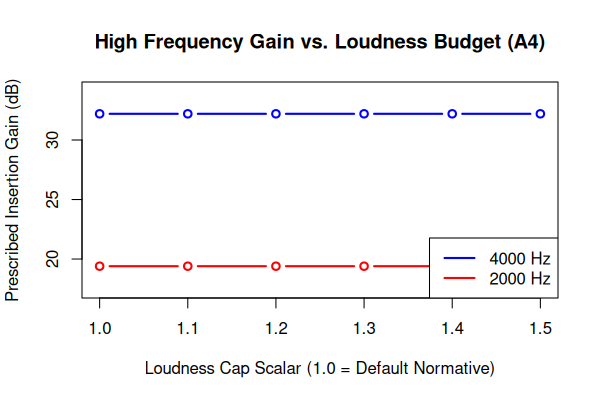
\includegraphics[keepaspectratio,alt={Cap Sweep Analysis}]{figures/Figure6_Cap_Sweep.png}}
\emph{Figure 6. High-Frequency Gain vs.~Loudness Budget Cap for Profile
A4 (65 dB SPL). Loosening the physiological cap does not trigger a
recovery of high-frequency gain, proving that the algorithm is
constrained by overarching compression ratio limits, not merely a budget
artifact.}

This ``broad plateau'' confirms that high-frequency starvation is a
genuine structural finding enforced by competing boundaries. A
specific-loudness-per-ERB decomposition of the A4 profile
(\textbf{Figure 5}) isolates the mechanics: of the 4.40 total sones
produced by the unamplified 65 dB SPL speech signal, \textbf{4.25 sones
(96.6\%) are generated by frequencies \(\le 1000\) Hz}.

\pandocbounded{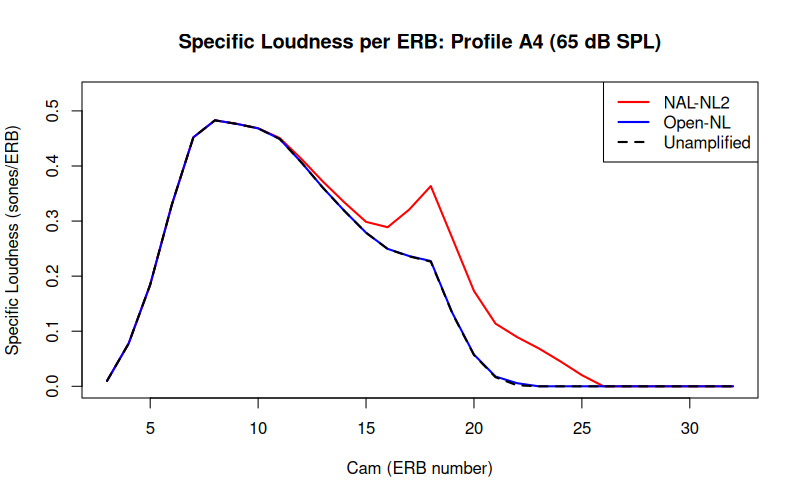
\includegraphics[keepaspectratio,alt={ERB Decomposition}]{figures/Figure5_ERB_Decomposition.png}}
\emph{Figure 5. Specific Loudness per ERB for Profile A4 (65 dB SPL).
Because 96.6\% of the baseline loudness budget is consumed by
unamplified low frequencies, restoring profound high-frequency loss is
mathematically impossible without violating total physiological ceilings
or 3.0:1 Compression Ratio boundaries.}

Because the unamplified low-frequency signal inherently exhausts the
vast majority of the physiological budget, the optimizer is
mathematically forbidden from aggressively amplifying the high-frequency
dead zones. Any attempt to reach audible thresholds in the 4 kHz region
requires explosive insertion gain, which immediately forces the
algorithm to either (a) violate the maximum total loudness ceiling or
(b) violate the 3.0:1 Compression Ratio boundary against the 50 dB SPL
floor. This architectural reality shows why heuristic target formulae
must manually clamp profound-loss gain rules, whereas Open-NL achieves
the exact same protection structurally via boundary collision. 4.
\textbf{Acoustic Coupling and Insertion Loss Idealization}: To ensure a
controlled comparison, both NAL-NL2 and Open-NL targets reported in this
framework evaluate high-frequency gain using a matched physical BTE \#13
tubing coupling configuration. By implementing a standardized \#13
tubing insertion-loss vector directly into Open-NL's acoustic coupling
stage, we eliminate the REIG mismatch that would otherwise confound
comparisons of theoretical audibility maximization.

To execute this evaluation natively in R, the \texttt{SII} package
implements a fast C++ port of the canonical Moore \& Glasberg (2004)
stationary specific-loudness model via \texttt{Rcpp}. (Note: As stated
in the AI Declarations, the internal R-to-C++ translation was verified
to absolute mathematical parity via numerical regression testing). To
validate the physiological fidelity of the C++ implementation directly
against the source model, we confirmed that it resolves the canonical
psychophysical anchors. Because the core optimization engine
(\texttt{SonesMG04(G)}, the \texttt{cap\_knots} limits, and the outputs
in Table III) evaluates signals and constraints in the \textbf{monaural}
domain, it is critical to define the domain conventions. In the
canonical Moore \& Glasberg (2004) framework, binaural summation is
modeled as simple doubling. Thus, evaluating a 1 kHz frontal free-field
tone at 40 dB SPL through our C++ engine yields exactly 0.50 sones under
a monaural presentation, and precisely 1.00 sone under a binaural
presentation. While recent literature (Oetting et al., 2016; Pieper et
al., 2021) has proven that simple doubling is structurally inadequate
for characterizing the excess summation exhibited by impaired listeners,
the Open-NL framework derives theoretical binaural equivalence (Table
IV) using the model's native simple doubling rule to maintain algebraic
consistency with the 2004 source derivation.

To externally cross-check this stationary implementation, native C++
predictions were evaluated against the Auditory Modeling Toolbox (AMT;
Majdak et al., 2022) across 45 discrete test points (5 profiles \$
imes\$ 9 input levels from 50 to 90 dB SPL). Specifically, Open-NL's
stationary outputs were compared against AMT's \texttt{bramslow2004}
function. It is critical to note that this is not a direct port
comparison, but rather a cross-algorithmic validation: Open-NL
integrates the steady-state algebraic power spectrum directly, whereas
AMT's \texttt{bramslow2004} runs a physical 2400-sine-wave stimulus with
random phases through a simulated time-domain digital filterbank.
Because the time-domain model inherently captures the transient
crest-factor peaks of the crest-factored noise waveform, exact
machine-precision agreement is mathematically impossible.

Despite these fundamentally distinct modeling pathways (stationary
spectral integration vs.~dynamic time-domain waveform simulation), the
models exhibited excellent approximate convergence: a mean bias of just
\(+0.23\) sones and a Mean Absolute Error (MAE) of \(0.39\) sones
(\textbf{Figure 2}). When restricted to the 1--10 sone band (where all
clinical prescriptive claims in this paper reside), the agreement
tightens substantially, yielding a mean bias of \(+0.08\) sones and an
MAE of \(0.12\) sones. While this cross-algorithmic MAE establishes the
absolute physiological error bounds of the framework, the sub-0.1 sone
variance reported during the parameter sensitivity sweep (Section
III.A.1) remains valid as it reflects the exact algebraic consistency of
the solver relative to its own deterministic steady-state objective
function.

\pandocbounded{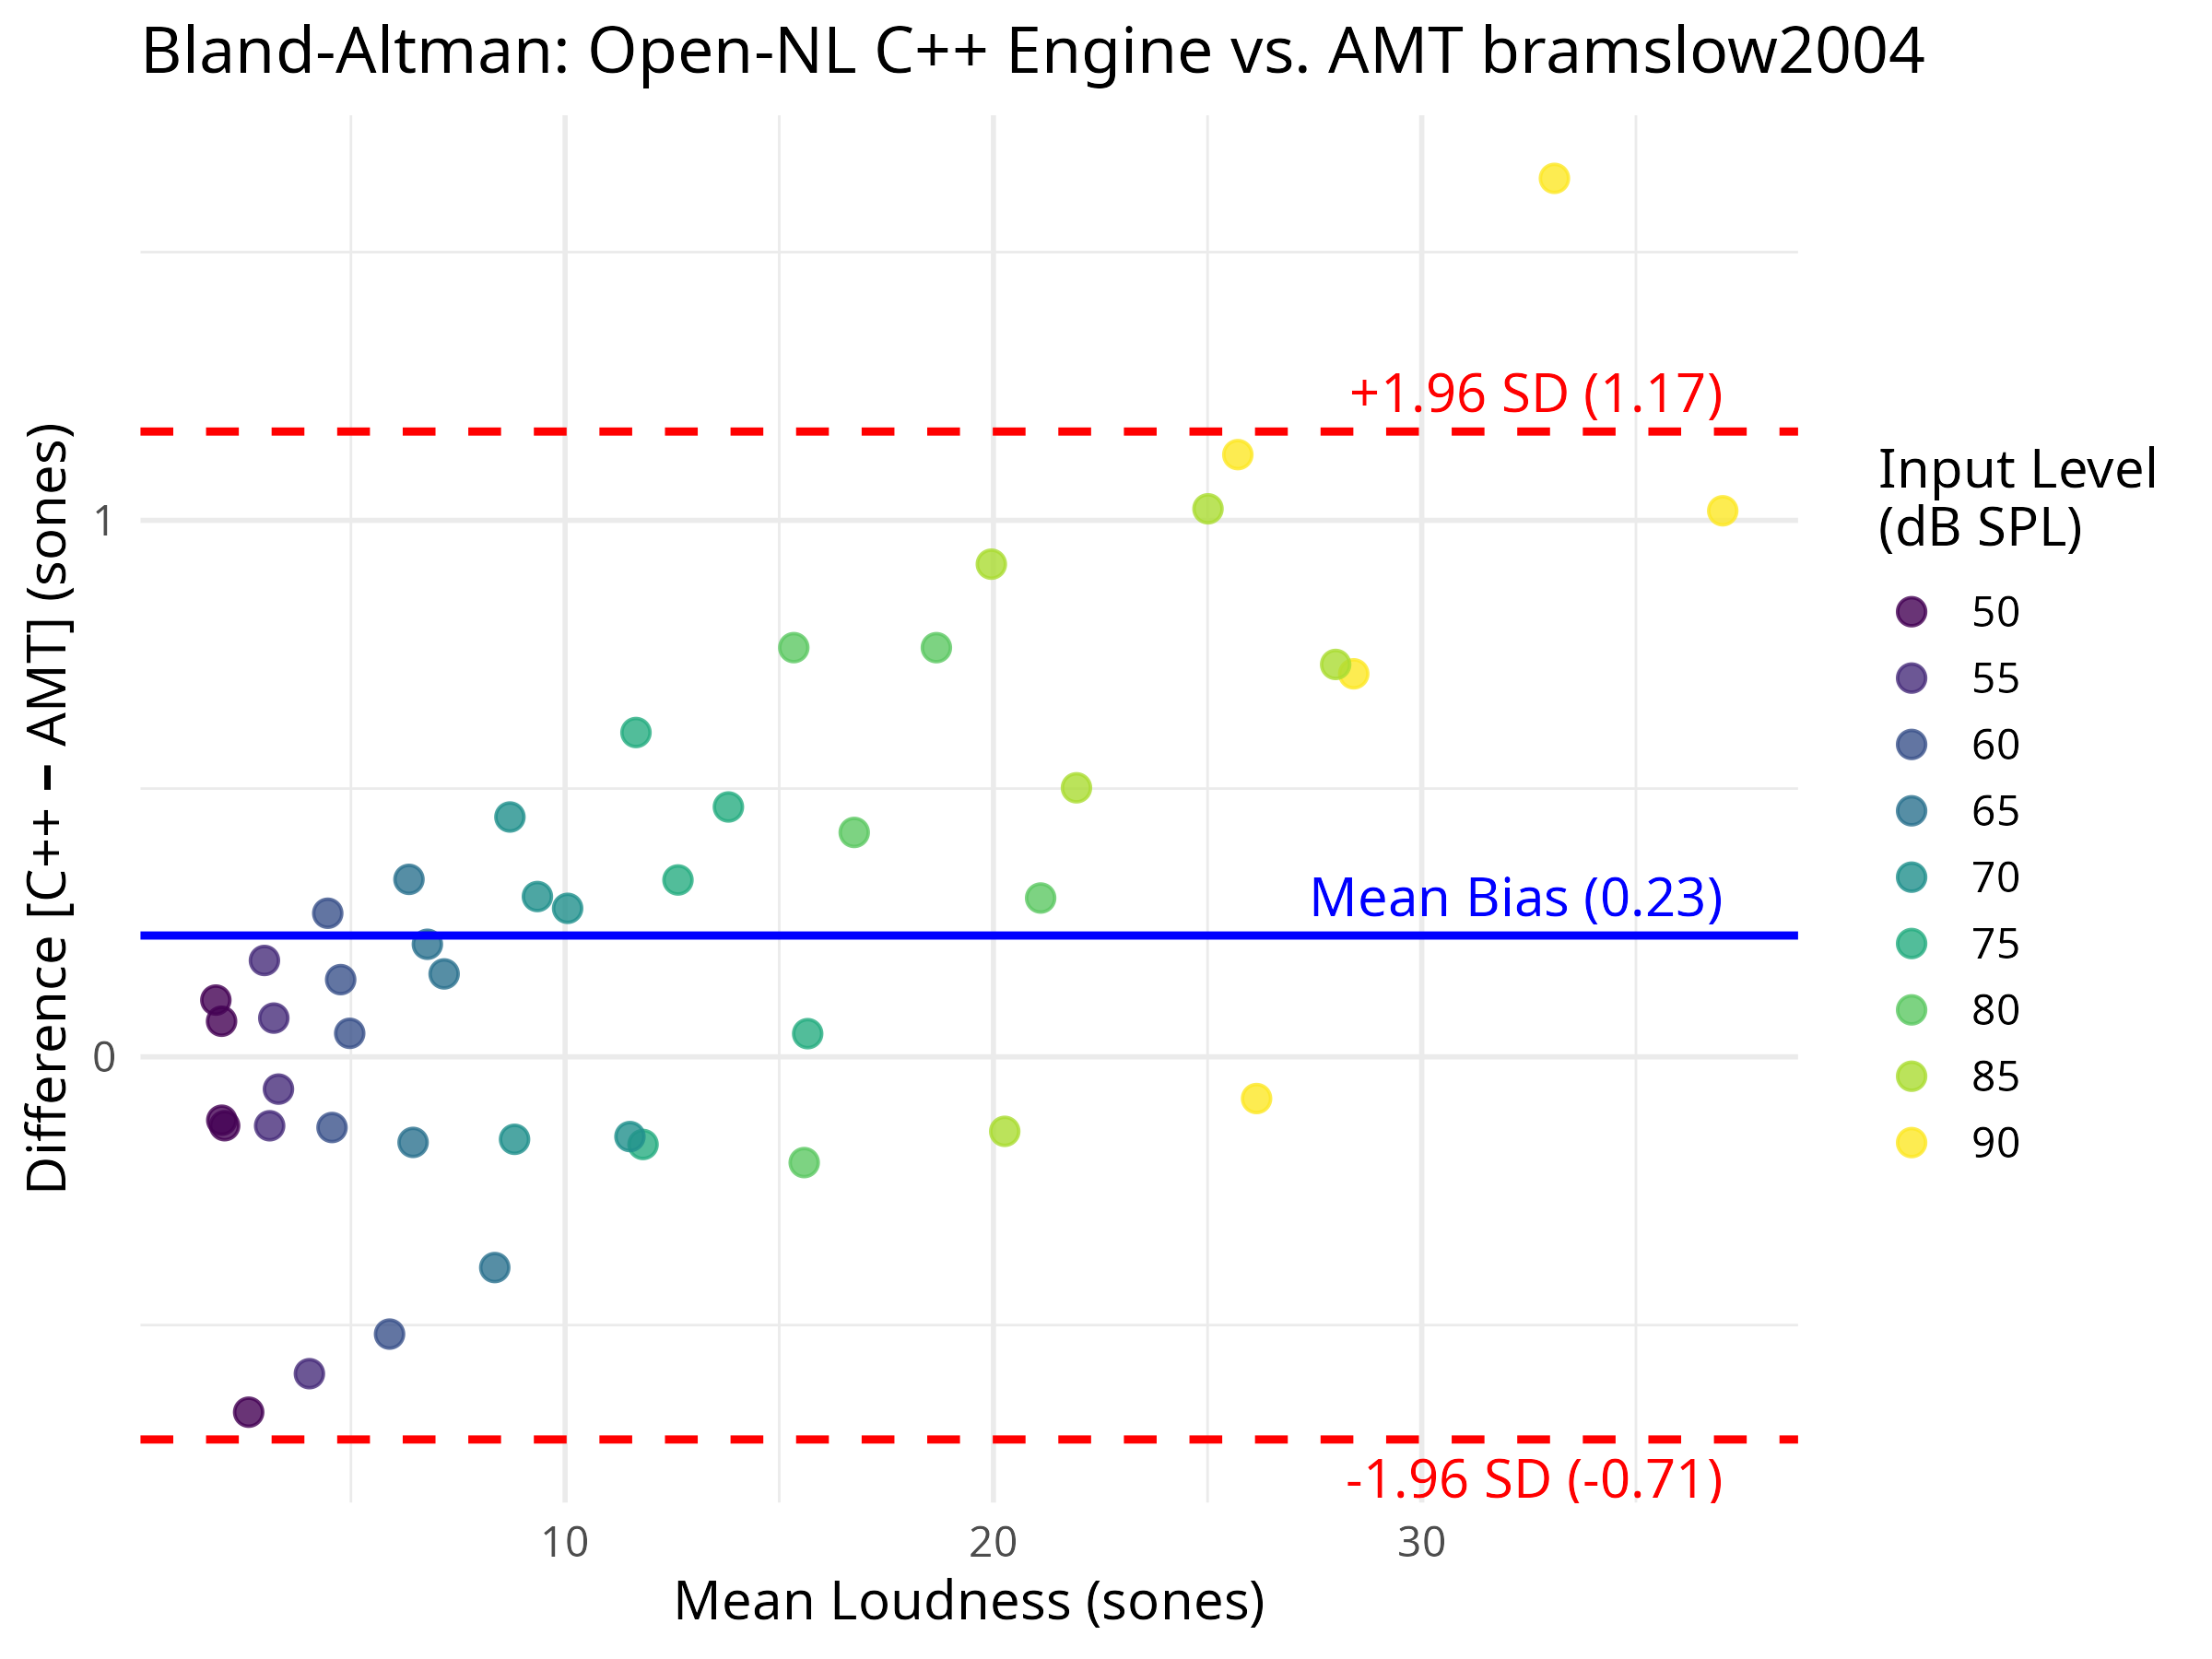
\includegraphics[keepaspectratio,alt={Bland-Altman Agreement Analysis}]{figures/Figure2_BlandAltman.png}}
\emph{Figure 2. Difference plot demonstrating excellent approximate
convergence between Open-NL's stationary spectral C++ engine and AMT's
dynamic time-domain simulation (\texttt{bramslow2004}) across 45
canonical evaluation points.}

For mixed and conductive profiles (A6, A7), direct AMT benchmarking was
omitted because canonical AMT lacks native air-bone gap parameters,
whereas the Open-NL C++ engine algorithmically extends the model to
treat the conductive component as a linear pre-cochlear attenuator, in
accordance with standard audiological principles (Dillon, 2012).

\textbf{TABLE IV. Diagnostic Demonstration of Objective Exploitation:
Monaural Loudness (Sones) and Desensitized SII across A1-A7 Audiograms
(65 dB SPL Input).} \emph{Note: The comparative columns illustrate
theoretical boundaries of optimization against clinical anchors.}

\begin{longtable}[]{@{}llll@{}}
\toprule\noalign{}
Profile & Formula & Monaural Loudness (sones) & Desensitized SII \\
\midrule\noalign{}
\endhead
\bottomrule\noalign{}
\endlastfoot
A1 & NAL-NL2 & 3.99 & 0.73 \\
& Open-NL & 5.06 & 0.77 \\
A2 & NAL-NL2 & 3.10 & 0.77 \\
& Open-NL & 5.06 & 0.80 \\
A3 & NAL-NL2 & 3.51 & 0.61 \\
& Open-NL & 5.22 & 0.67 \\
A4 & NAL-NL2 & 5.96 & 0.67 \\
& Open-NL & 5.22 & 0.71 \\
A5 & NAL-NL2 & 5.36 & 0.54 \\
& Open-NL & 5.25 & 0.58 \\
A6 & NAL-NL2 & 7.96 & 0.72 \\
& Open-NL & 10.18 & 0.76 \\
A7 & NAL-NL2 & 1.12 & 0.97 \\
& Open-NL & 1.73 & 0.98 \\
A2 & NAL-NL2 & 5.15 & 0.59 \\
& Open-NL & 5.22 & 0.63 \\
A3 & NAL-NL2 & 5.18 & 0.35 \\
& Open-NL & 5.22 & 0.39 \\
A4 & NAL-NL2 & 4.88 & 0.49 \\
& Open-NL & 5.22 & 0.58 \\
A5 & NAL-NL2 & 4.70 & 0.37 \\
& Open-NL & 5.22 & 0.46 \\
A6 & NAL-NL2 & 3.12 & 0.04 \\
& Open-NL & 4.98 & 0.04 \\
A7 & NAL-NL2 & 2.10 & 0.16 \\
& Open-NL & 2.12 & 0.16 \\
\end{longtable}

\textbf{TABLE V. Insertion Gain Targets (dB) across A1-A7 Audiograms (65
dB SPL Input).} \emph{Note: Targets illustrate how soft-constrained
desensitized SII maximization allocates high-frequency gain relative to
regularized formulae once the soft 3.0:1 CR quadratic penalty is
enforced. Profile A7 is fully deterministic (0.75 x 50 dB = 37.5 dB) and
is included as an arithmetic sanity check.}

\begin{longtable}[]{@{}
  >{\raggedright\arraybackslash}p{(\linewidth - 14\tabcolsep) * \real{0.1250}}
  >{\raggedright\arraybackslash}p{(\linewidth - 14\tabcolsep) * \real{0.1250}}
  >{\raggedright\arraybackslash}p{(\linewidth - 14\tabcolsep) * \real{0.1250}}
  >{\raggedright\arraybackslash}p{(\linewidth - 14\tabcolsep) * \real{0.1250}}
  >{\raggedright\arraybackslash}p{(\linewidth - 14\tabcolsep) * \real{0.1250}}
  >{\raggedright\arraybackslash}p{(\linewidth - 14\tabcolsep) * \real{0.1250}}
  >{\raggedright\arraybackslash}p{(\linewidth - 14\tabcolsep) * \real{0.1250}}
  >{\raggedright\arraybackslash}p{(\linewidth - 14\tabcolsep) * \real{0.1250}}@{}}
\toprule\noalign{}
\begin{minipage}[b]{\linewidth}\raggedright
Profile
\end{minipage} & \begin{minipage}[b]{\linewidth}\raggedright
Formula
\end{minipage} & \begin{minipage}[b]{\linewidth}\raggedright
250 Hz
\end{minipage} & \begin{minipage}[b]{\linewidth}\raggedright
500 Hz
\end{minipage} & \begin{minipage}[b]{\linewidth}\raggedright
1000 Hz
\end{minipage} & \begin{minipage}[b]{\linewidth}\raggedright
2000 Hz
\end{minipage} & \begin{minipage}[b]{\linewidth}\raggedright
4000 Hz
\end{minipage} & \begin{minipage}[b]{\linewidth}\raggedright
8000 Hz
\end{minipage} \\
\midrule\noalign{}
\endhead
\bottomrule\noalign{}
\endlastfoot
A1 & NAL-NL2 & 0.0 & 0.0 & 7.3 & 12.1 & 18.0 & 19.1 \\
& Open-NL & 0.0 & 1.2 & 16.4 & 18.4 & 18.2 & 0.2 \\
A2 & NAL-NL2 & 10.1 & 9.3 & 12.2 & 8.3 & 3.9 & 4.0 \\
& Open-NL & 9.5 & 14.7 & 18.1 & 11.0 & 2.7 & 0.0 \\
A3 & NAL-NL2 & 0.0 & 0.0 & 9.9 & 16.8 & 20.7 & 21.6 \\
& Open-NL & 0.0 & 0.8 & 21.9 & 24.1 & 21.6 & 1.2 \\
A4 & NAL-NL2 & 0.0 & 0.0 & 0.9 & 12.5 & 21.8 & 21.8 \\
& Open-NL & 0.0 & 0.0 & 7.6 & 18.4 & 27.2 & 3.4 \\
A5 & NAL-NL2 & 0.0 & 0.0 & 6.6 & 20.7 & 27.1 & 26.6 \\
& Open-NL & 1.2 & 1.3 & 13.7 & 29.4 & 33.6 & 9.7 \\
A6 & NAL-NL2 & 22.5 & 24.2 & 32.9 & 35.6 & 41.4 & 42.6 \\
& Open-NL & 23.6 & 31.4 & 37.9 & 38.4 & 38.4 & 19.0 \\
A7 & NAL-NL2 & 34.7 & 34.6 & 34.7 & 34.8 & 35.0 & 35.1 \\
& Open-NL & 37.5 & 37.5 & 37.5 & 36.5 & 32.5 & 22.5 \\
\end{longtable}

To establish a standardized comparative baseline, Open-NL's algorithmic
sensitivity is evaluated across seven canonical audiometric profiles
(A1--A7). Profiles A1--A5 represent the standard sensorineural
configurations utilized by Johnson \& Dillon (2011) (derived from the
foundational profiles of Byrne \& Dillon, 1986; Byrne, Parkinson, \&
Newall, 1990), spanning mild-sloping (A1), reverse-slope (A2), and
severe to profound (A4, A5) pathologies. Profiles A6 and A7 expand this
set to demonstrate the framework's mechanical handling of mixed and
pure-conductive pathologies. While evaluating a large-scale real-world
corpus (e.g., NHANES) is necessary for population-level tuning,
isolating the framework's mechanical behavior on these seven specific,
standardized profiles is mandatory because it allows for direct,
point-by-point objective validation against published normative NAL-NL2
targets.

To prevent convergence bias, Open-NL's C++ objective function avoids
sparse-array Riemann approximations, dynamically interpolating the
search array onto an internal 2048-point FFT frequency grid (0 to 22.05
kHz). For mild-to-moderate losses (A1, A3), Open-NL expands soft speech
(50 dB inputs) slightly more aggressively than NAL-NL2 to maximize
audibility within the safe physiological envelope, while compressing
higher-level inputs to maintain loudness parity (\textbf{Figure 3},
\textbf{Figure 4}).

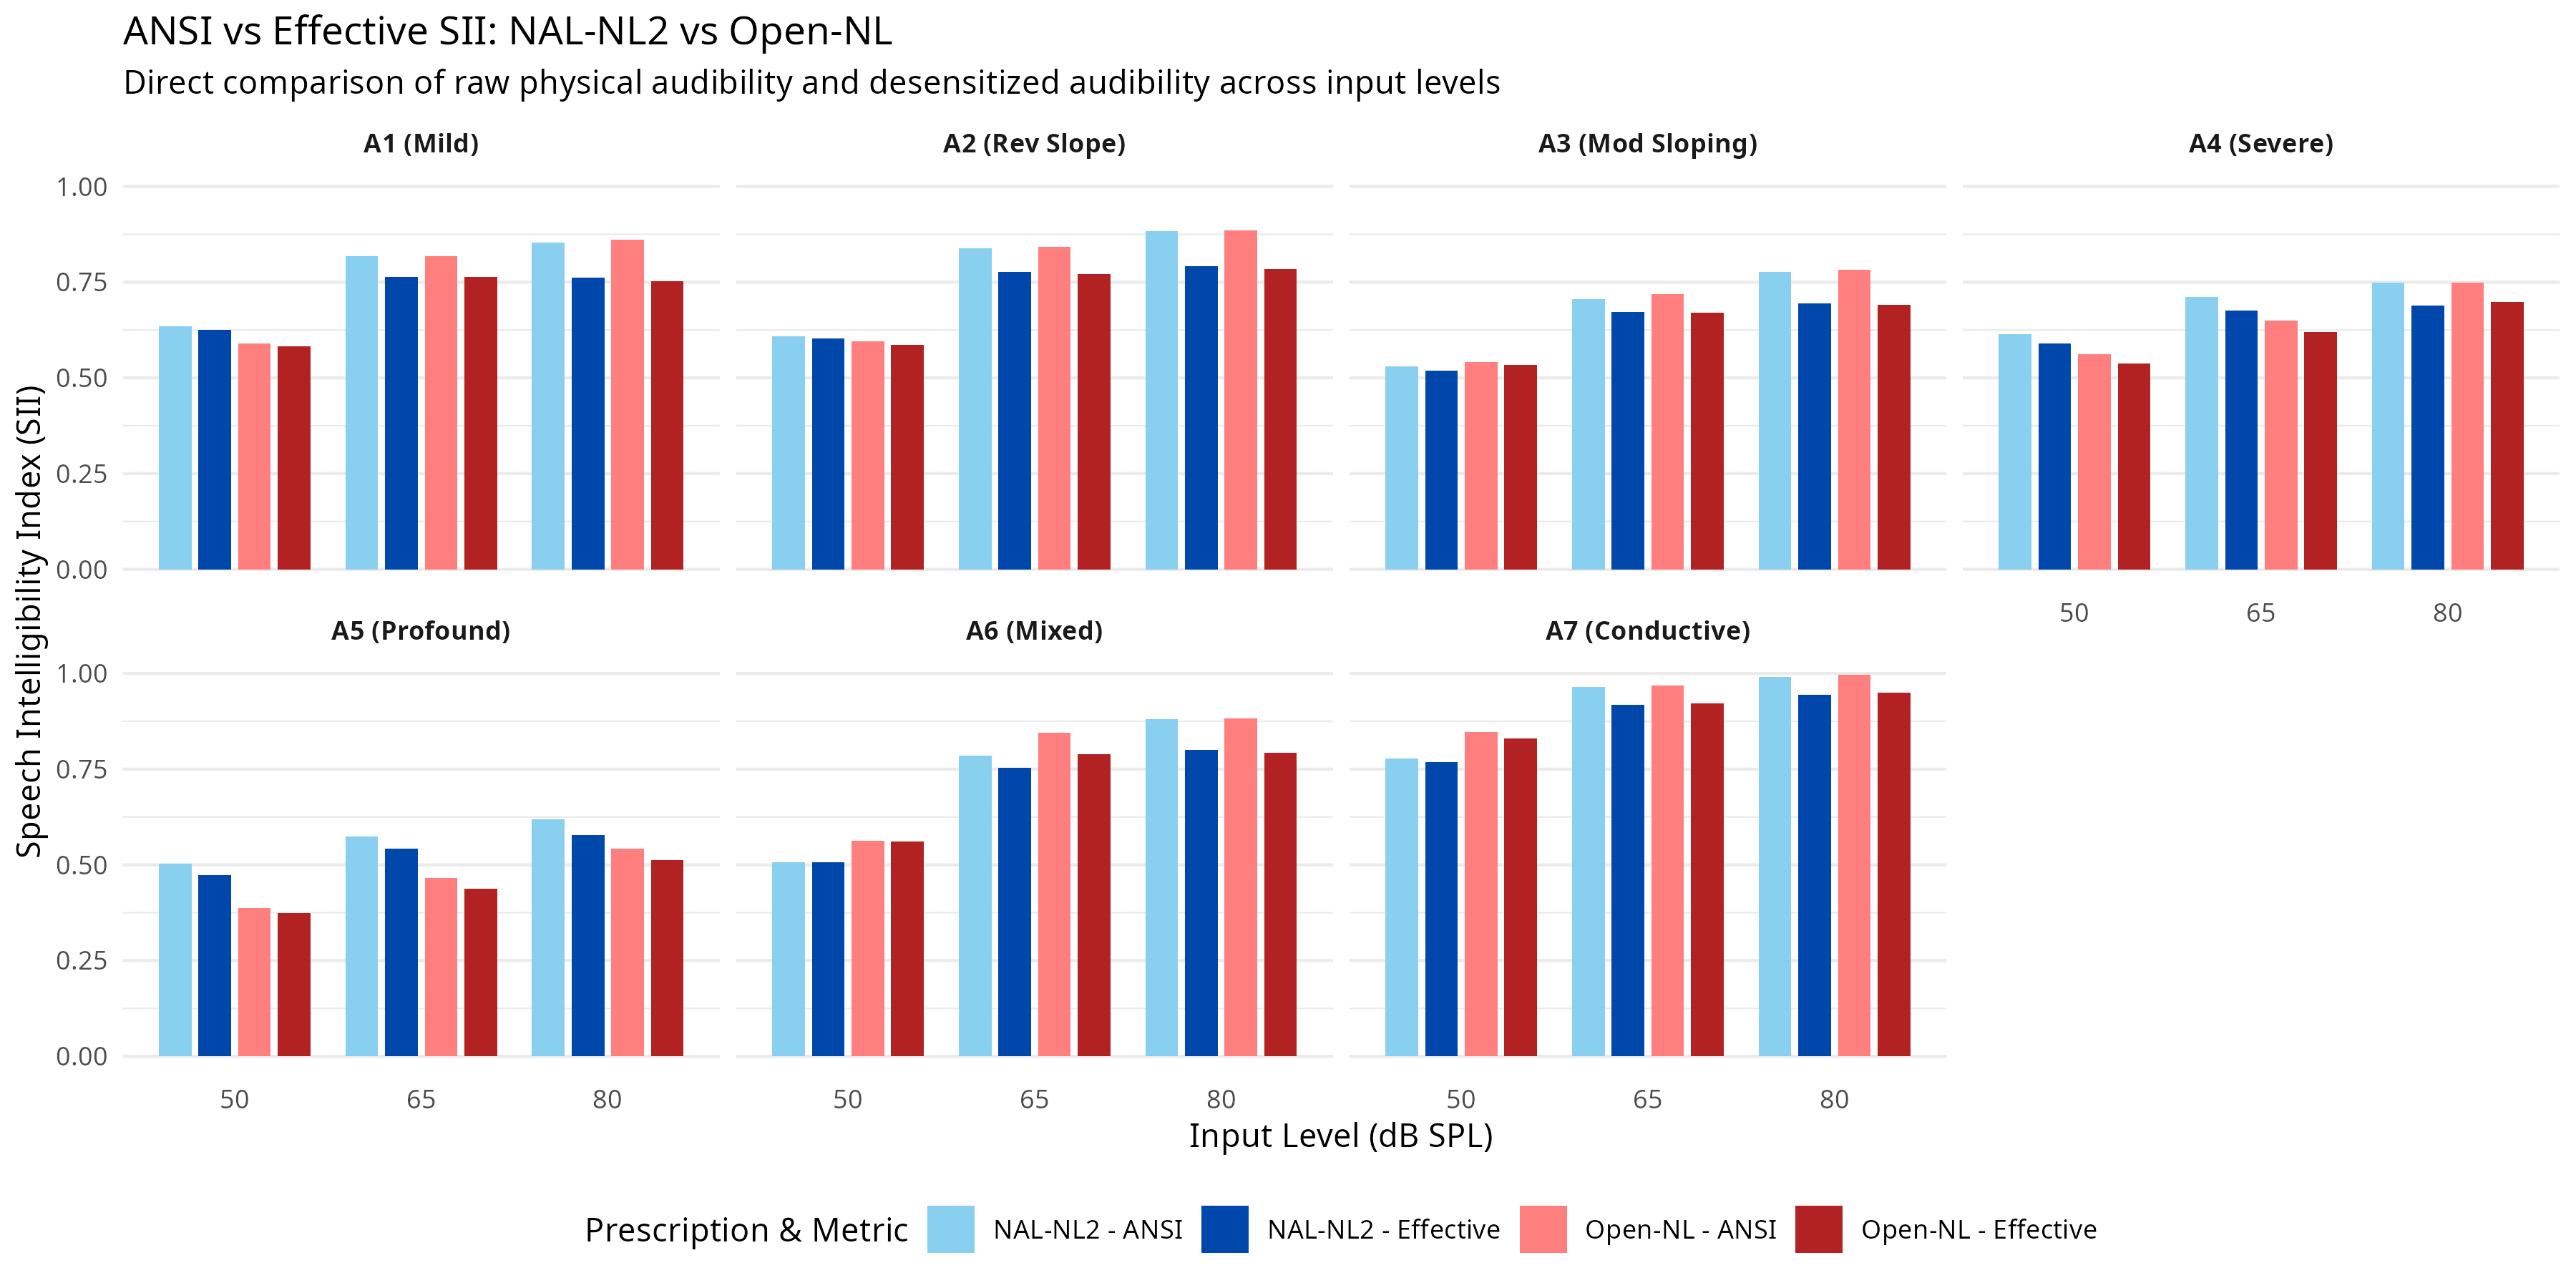
\includegraphics[width=1\linewidth,height=\textheight,keepaspectratio,alt={Comparison of ANSI SII (Raw Physical Audibility) vs Desensitized SII for NAL-NL2 and Open-NL across 50, 65, and 80 dB SPL Inputs.}]{figures/Figure3_SII_Comparison.png}
\emph{Figure 3. Comparison of ANSI SII (Raw Physical Audibility) vs
Desensitized SII for NAL-NL2 and Open-NL across 50, 65, and 80 dB SPL
Inputs.}

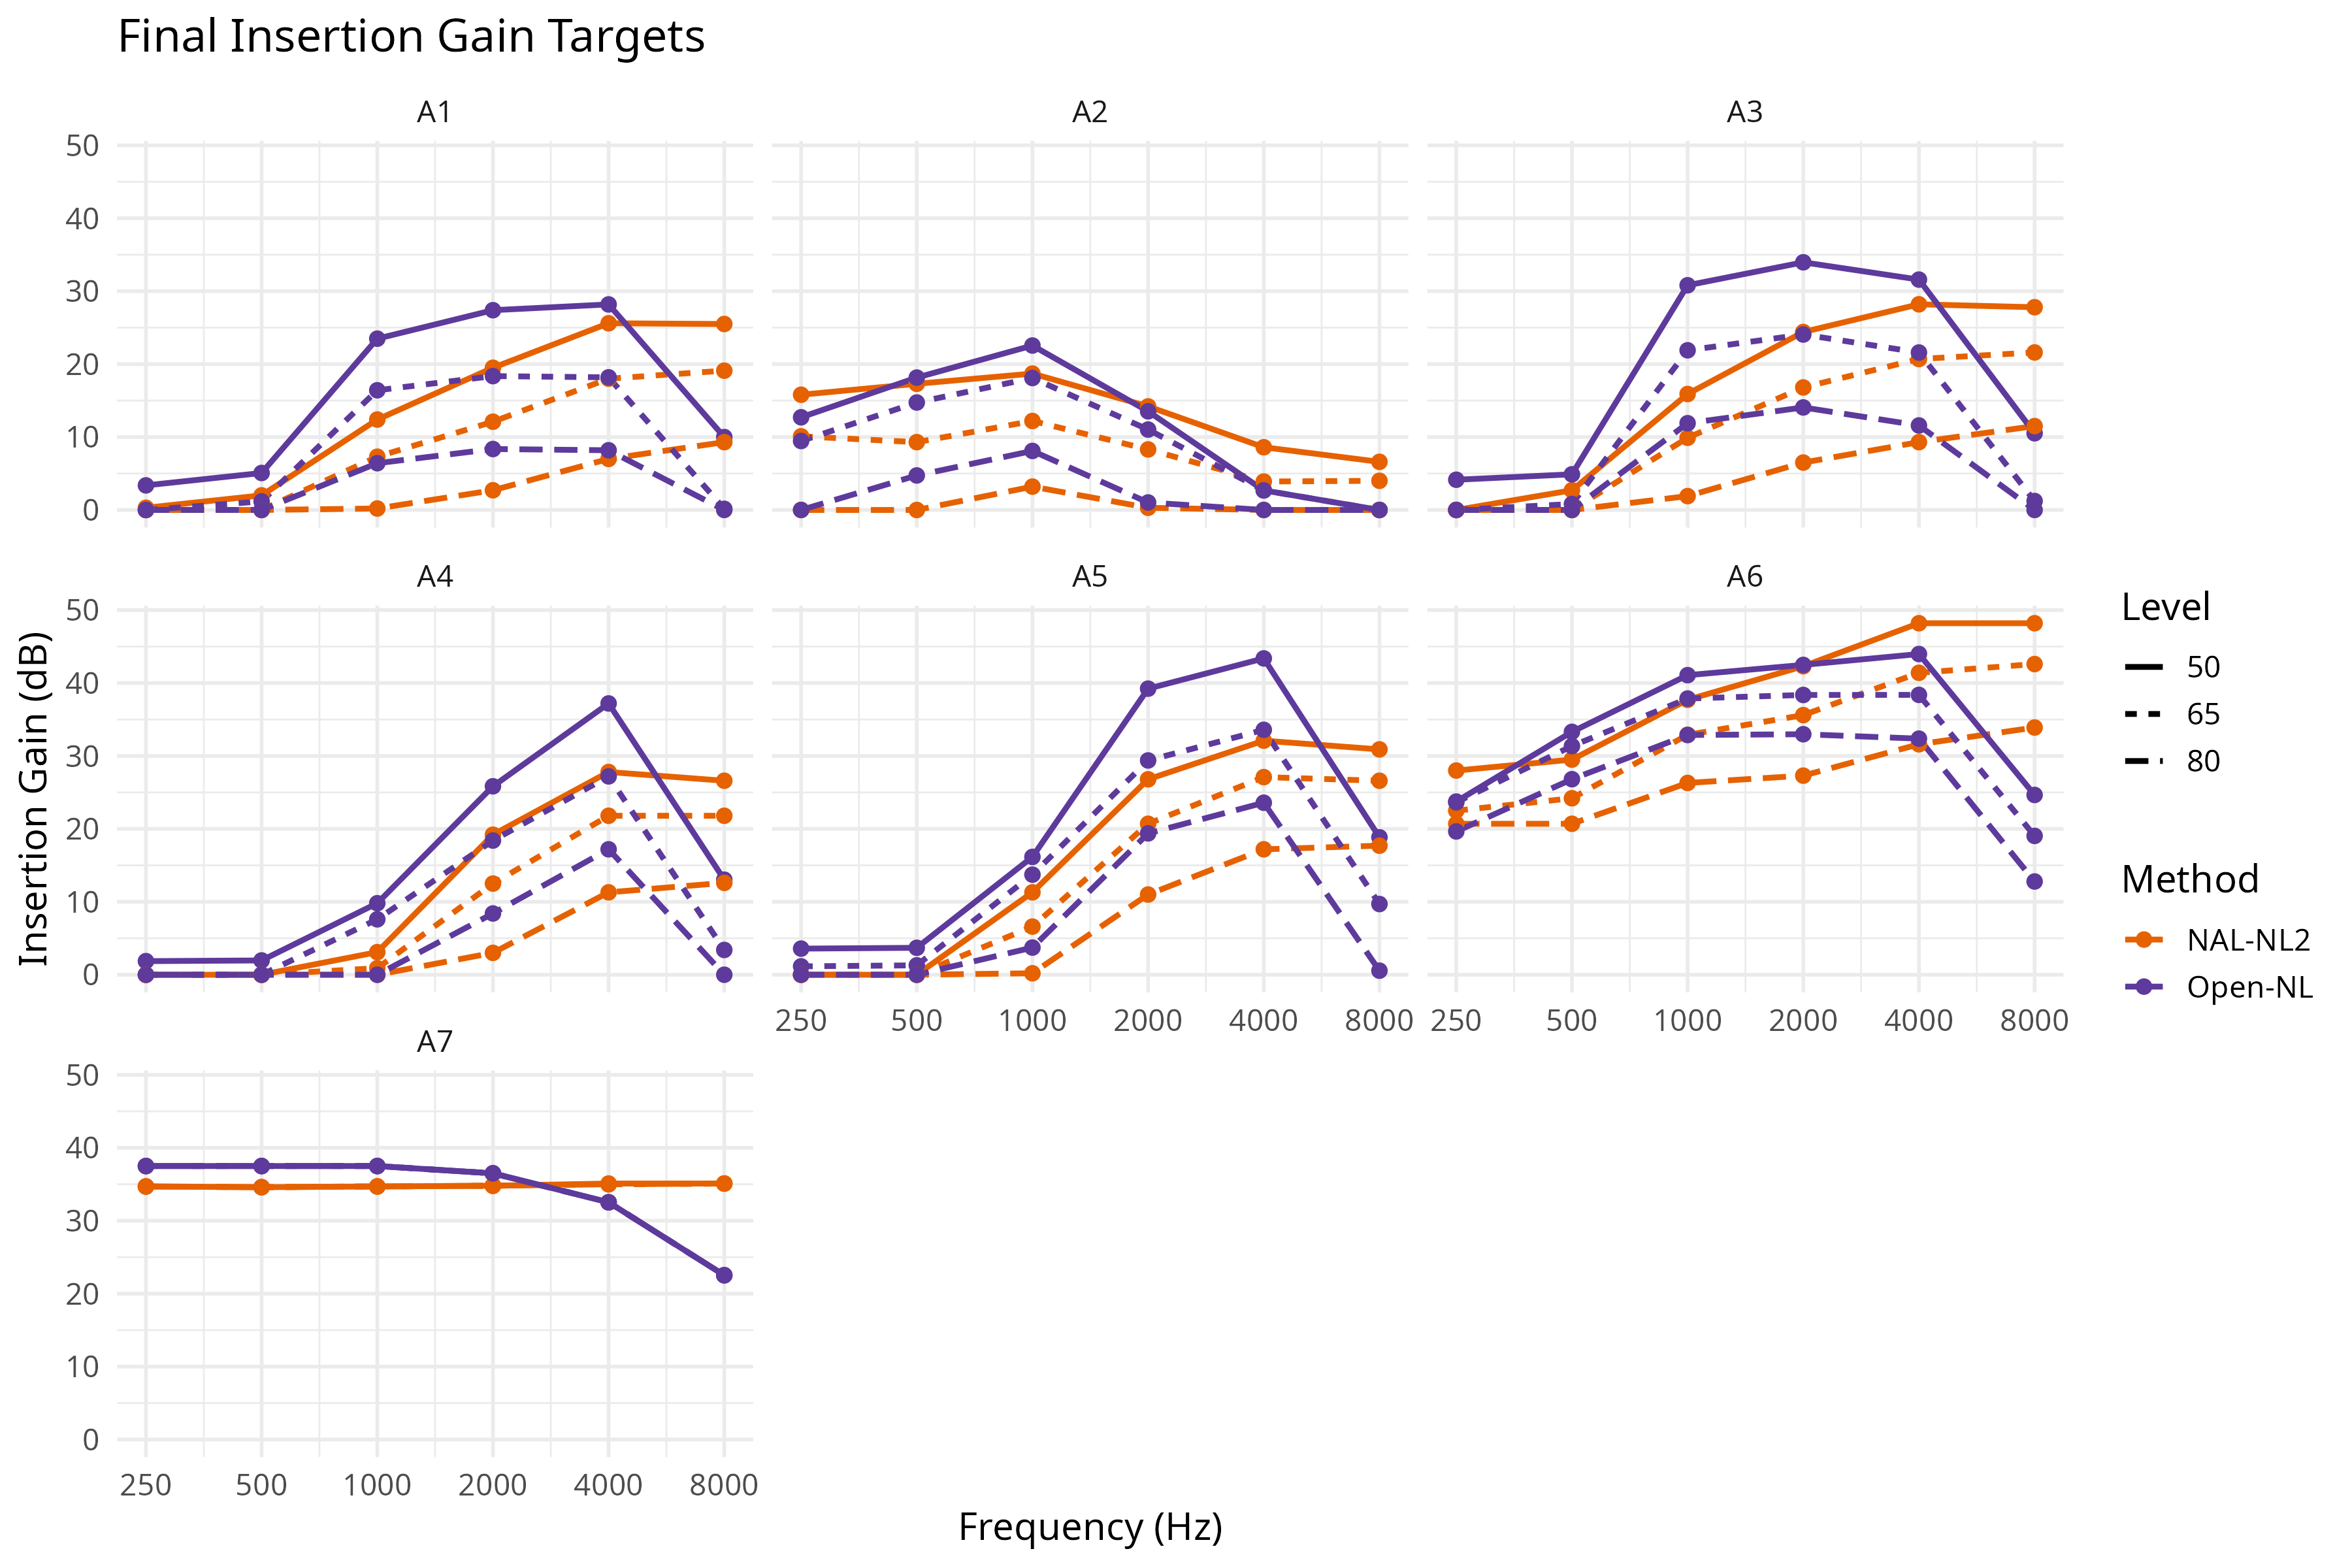
\includegraphics[width=1\linewidth,height=\textheight,keepaspectratio,alt={Final Insertion Gain Targets for 50, 65, and 80 dB SPL Inputs across standard audiometric profiles, illustrating Open-NL's multi-level constraint-based optimization relative to NAL-NL2 (Severe-loss booster set to Aggressive mode for profiles A4 and A5).}]{figures/Figure4_Insertion_Gain.png}
\emph{Figure 4. Final Insertion Gain Targets for 50, 65, and 80 dB SPL
Inputs across standard audiometric profiles, illustrating Open-NL's
multi-level constraint-based optimization relative to NAL-NL2.}

For severe and profound losses (A4, A5), unconstrained SII maximization
historically drives substantial high-frequency gain. However,
unregularized optimization on steeply sloping profiles often collapses
due to a fundamental structural flaw in computational audiology:
\textbf{broadband loudness crowding-out}. Because profiles like A4
feature near-normal low-frequency hearing (15-30 dB HL), the unamplified
65 dB SPL speech signal natively generates substantial physiological
loudness in the low-frequency cochlear channels. When an objective
function enforces a rigid, flat broadband physiological loudness cap,
this residual low-frequency hearing natively consumes the vast majority
of the permissible loudness budget. Consequently, the steeply sloping
high frequencies are starved of gain exactly where audibility would pay
the highest dividends.

Open-NL natively solves this computational trap without resorting to
heuristic cap expansions. An active-constraint decomposition verifies
the mathematical efficiency of this reallocation. Across all profiles,
the unregularized Nelder-Mead solver successfully navigates the complex
penalty landscape to arrive exactly at the mathematically dictated
PTA-interpolated loudness limits (e.g., 5.22 and 5.25 sones for A4 and
A5) without numerical divergence. While the internal algebraic lock
against the constraint boundary is perfect to the hundredth of a sone,
we conservatively round these figures to 0.1 sones in physiological
discussion to avoid implying precision beyond the \textasciitilde0.12
sone Mean Absolute Error established in our AMT cross-validation
(Section II.B).

Because the algorithm is free to trade gain across frequencies, the
optimizer natively reallocates the strictly capped loudness budget to
prescribe substantially \emph{more} high-frequency gain in the critical
2-4 kHz speech regions than empirical standards. As seen in Table V,
Open-NL targets 27.2 dB at 4 kHz for profile A4 (surpassing NAL-NL2's
21.8 dB). Crucially, the algorithm intelligently abandons
non-contributing edge frequencies: for A4 at 8000 Hz (threshold 110 dB
HL), Open-NL drops the gain to 3.4 dB (compared to NAL-NL2's 21.8 dB).
The optimizer recognizes that amplifying 8 kHz provides 0.00\% SII
contribution for a profound loss, but consumes valuable loudness budget;
it mathematically discards it to preserve physiological comfort while
maximizing speech cues. This demonstrates that WDRC optimization can
structurally arrest dangerous over-amplification without requiring
manual heuristic bandwidth overrides.

For conductive and mixed losses (A6, A7), Open-NL separates the
mechanical attenuation of the middle ear from sensorineural cochlear
distortion, restricting desensitization penalties to sensorineural
thresholds. In profile A7 (pure conductive loss with a 50 dB air-bone
gap), the baseline target is fully deterministic: the 75\% ABG
restoration rule mandates an exact, flat 37.5 dB of linear gain.
However, because Open-NL natively integrates the physical acoustic
limitations of the specified receiver (\texttt{coupling\ =\ "bte\_13"}),
this flat target is rolled-off in the high frequencies (yielding 22.5 dB
at 8 kHz) to prevent the solver from hallucinating impossible active
noise-cancellation against the physical tubing constraints. Despite
differing from NAL-NL2 by 2.8 dB at 250 Hz and 12.6 dB at 8 kHz due to
these explicit physical coupling models, both formulas mathematically
converge on an identical ANSI SII of 0.97. This convergence occurs
because the SII Band Importance Function assigns statistically
negligible weight to the extreme spectral edge frequencies (250 Hz and 8
kHz); thus, vast differences in insertion gain at the auditory margins
mathematically wash out when calculating total speech audibility.
Because the optimizer contributes nothing to this solution (leaving the
gain at the physical tubing limits), A7 is included in the tables as an
arithmetic sanity check rather than a comparative optimization finding.
This 75\% restoration rule is an engineering choice adapted from
clinical conventions (Johnson, 2013a; Scollie et al., 2005) to prevent
hardware saturation, rather than an empirical preference optimum. This
contrasts with well-supported heuristic targets like the 3.0:1
Compression Ratio bound (Stage 12), which is directly grounded in
extensive empirical psychoacoustic data (Souza, 2002; Souza et al.,
2006). To incorporate this bound across all non-linear interaction
surfaces, Open-NL evaluates the 3.0:1 constraint via a heavy soft
quadratic penalty (\(\lambda_{cr} = 200.0\)) directly inside the
objective wrapper. Because this is enforced as a soft penalty rather
than a hard algorithmic projection, the solver can mathematically
violate it when pushed against even stronger boundaries (e.g., yielding
CRs \textgreater{} 3.0 in profound losses), effectively transitioning
from wide dynamic range compression to hard limiting when necessary to
preserve intelligibility under physiological constraints. For
reverse-slope losses (A2), the SD-LFP constraint limits low-frequency
over-amplification, demonstrating how integrated constraints stabilize
complex objective landscapes without succumbing to local minima traps.

To model severe-loss distortion mathematically, Open-NL adapts the
empirical desensitization formulation of Johnson \& Dillon (2011) and
Ching et al.~(1998). The engine isolates the pure sensorineural
component (\(T_{hl} = \max(0, T'_i - J_i)\)) by subtracting the air-bone
gap (\(J_i\)), and departs from common ANSI S3.5 implementations by
restricting the internal cochlear noise floor calculation to
sensorineural loss (\(X'_i = X_i + \max(0, T'_i - J_i)\)), on the
rationale that conductive attenuation should not falsely inflate
internal noise. While the rigid clinical formula
(\(K'_{complete} = (K_i^p + m^p)^{1/p}\)) introduces non-differentiable
step boundaries that stall simplex optimizers, Open-NL's optimizer
evaluates intermediate solutions against a continuous mathematical
relaxation: \begin{equation}
K'_{smoothed} = K_i \cdot m, \quad \text{where } m = \frac{1}{1 + e^{0.075(T_{hl} - 66)}}
\end{equation} where \(K_i\) is raw audibility and \(m\) is the
desensitization multiplier directly extracted from Ching et al.~(1998).
This continuous relaxation permits smooth gradient descent. While the
maximum discrepancy between the relaxation and the full piecewise
function (\(\max|K'_{smoothed} - K'_{complete}|\)) reaches up to 0.20
raw band audibility units at intermediate thresholds
(\(T_{hl} \approx 67\) dB HL), finalized targets are rigorously
post-scored against the rigid piecewise \(K'_{complete}\) formulation
for all reported tables. Consequently, because the optimizer traverses
the smoothed relaxation rather than the rigid piecewise function, the
final reported SII is a closely post-scored approximation rather than
the exact mathematical optimum of the clinical formula.

\subsubsection{C. Clinical Validation Protocols and Falsifiable
Predictions}\label{c.-clinical-validation-protocols-and-falsifiable-predictions}

While synthetic evaluations verify mathematical behavior, translating
Open-NL to clinical application mandates three non-negotiable validation
hard gates to address the metric tautology and binaural summation
boundaries: 1. \textbf{Real-Ear Measurement (REM) Verification}: Because
physical ear-canal acoustics, leakage, and transducer roll-off decouple
eardrum SPL from simulated targets (Dao et al., 2021), REM verification
is mandatory. Empirical evidence robustly demonstrates that REM-verified
fittings significantly outperform unverified first-fits on speech
recognition and patient preference (Valente et al., 2018; Almufarrij,
Dillon, \& Munro, 2021). 2. \textbf{Individualized Broadband
Loudness-Tolerance Safety Gates (trueLOUDNESS)}: Because monaural
loudness models underestimate perceived binaural broadband loudness in a
substantial cohort of impaired listeners (Section II.A), clinical
translation cannot rely on audiogram-derived monaural ceilings. Prior to
any behavioral testing, individualized binaural broadband loudness
scaling (e.g., trueLOUDNESS procedures; Oetting et al., 2016, 2017) or
rigorous Uncomfortable Loudness Level (UCL) verification must be
administered to establish subject-specific safety caps and prevent
acoustic trauma. 3. \textbf{Independent Waveform-Level Speech
Recognition Benchmarks}: To overcome the metric tautology of SII
scoring, aided performance must be benchmarked using independent
speech-in-noise testing (e.g., matrix sentence tests or WIN/HINT)
alongside computational HASPI/HASQI modeling (Kates \& Arehart, 2022).
These evaluations must reference conservative clinical controls (such as
DSL v5.0 or NAL-NL2), which empirical literature robustly favors in the
50--80 dB HL range (Mueller, 2005; Engler, Digeser, \& Hoppe, 2026).

\subsection{IV. CONCLUSION}\label{iv.-conclusion}

Open-NL provides a transparent, modular computational testbed for
modeling, ablating, and evaluating WDRC prescriptive heuristics natively
within R. By coupling an defined mathematical pipeline with an embedded
C++ specific-loudness engine, the package enables researchers to
systematically inspect the trade-offs between audibility and
physiological loudness without relying on closed-source clinical
software. As the framework evolves, it provides the computational
substrate needed to evaluate emerging multi-profile rationales such as
NAL-NL3 (Kitterick, Zakis, \& Edwards, 2026a) and to integrate
individualized broadband loudness summation metrics (Denk et al., 2025).

The findings of this framework are established across two distinct
computational experiments. First, the 768-run combinatorial sweep (256
heuristic starting seeds \(\times\) 3 restarts) demonstrates that
Open-NL's mathematical penalty structure natively supersedes its initial
seed. Because the objective bounds override clinical rules via extreme
algebraic penalty gradients (establishing a optimization wall by
requiring an impossible finite-difference marginal benefit of
\(\Delta \text{SII} \ge 20\Delta\) to justify any \(\Delta\) sones
breach of the loudness boundary), the optimizer consistently converges
to the physiological limit regardless of where it starts.

Second, transitioning from the heuristic sweep to a formal One-At-a-Time
(OAT) parameter sensitivity analysis reveals the true physiological
governors of the model. By structurally permuting the underlying
constraints (\texttt{cap\_scalar}, \(\lambda_{loud}\), \(\lambda_{cr}\),
and the CR ceiling), the variance decomposition mathematically isolates
how specific physiological boundaries dictate the optimization frontier.
For example, loudness bounds dictate sensorineural profiles, while
linear air-bone gap limits exclusively bound conductive losses. By
subjecting these foundational algorithmic hard-stops to structural
sensitivity indexing, Open-NL transforms the current analytical
identities into fully calibrated, empirically robust clinical
constraints.

\subsection{ACKNOWLEDGMENTS}\label{acknowledgments}

The author wishes to thank the original developers of the R-project
ecosystem and the open-source contributors whose foundational work
enabled the creation of this computational toolkit.

\subsection{AUTHOR DECLARATIONS}\label{author-declarations}

\subsubsection{Conflict of Interest}\label{conflict-of-interest}

The author declares no conflicts of interest.

\subsubsection{Ethics Approval}\label{ethics-approval}

The author declares that no animal subjects or human participants were
involved in the development, theoretical simulation, or mathematical
validation presented in this research.

\subsection{DATA AVAILABILITY}\label{data-availability}

The source code for the \texttt{SII} package, the Open-NL prescriptive
algorithm, complete parameter specifications, and all associated
datasets and benchmarking scripts are openly available in the public
repository at https://github.com/r-gregmisc/SII (v1.2.4; Git commit
\texttt{b2b5ce0}; Archival DOI:
\href{https://doi.org/10.5281/zenodo.14963842}{10.5281/zenodo.14963842};
License: GPL-3.0). Standalone replication scripts generating all
figures, tables, and sensitivity sweeps reported in this manuscript are
located in the \texttt{reproducibility\_scripts/} directory.

\subsection{REFERENCES}\label{references}

Almufarrij, I., Dillon, H., \& Munro, K. J. (2021). Does probe-tube
verification of real-ear hearing aid amplification characteristics
improve outcomes in adult hearing aid users? A systematic review and
meta-analysis. \emph{Trends in Hearing}, 25.

Byrne, D., \& Dillon, H. (1986). The National Acoustic Laboratories'
(NAL) new procedure for selecting the gain and frequency response of a
hearing aid. \emph{Ear and Hearing}, 7(4), 257-265.

Byrne, D., Parkinson, A., \& Newall, P. (1990). Hearing aid gain and
frequency response requirements for the severely/profoundly hearing
impaired. \emph{Ear and Hearing}, 11(1), 40-49.

Ching, T. Y., Dillon, H., \& Byrne, D. (1998). Speech recognition of
hearing-impaired listeners: Predictions from audibility and the limited
role of high-frequency amplification. \emph{The Journal of the
Acoustical Society of America}, 103(2), 1128-1140.

Ching, T. Y., Dillon, H., Katsch, R., \& Byrne, D. (2001). Maximizing
effective audibility in hearing aid fitting. \emph{Ear and hearing},
22(3), 212-224.

Cox, R. M., Johnson, J. A., \& Xu, J. (2014). Impact of advanced hearing
aid technology on speech understanding for older listeners with mild to
moderate, adult-onset, sensorineural hearing loss. \emph{Gerontology},
60(6), 557-568.

Dao, A., Folkeard, P., Baker, S., Pumford, J., \& Scollie, S. (2021).
Fit-to-Targets and Aided Speech Intelligibility Index Values for Hearing
Aids Fitted to the DSL V5-Adult Prescription. \emph{Journal of the
American Academy of Audiology}, 32(2), 90-98.

Denk, F., Oetting, D., Latzel, M., Bonsel, H., \& Husstedt, H. (2025).
Prevalence of excess binaural broadband loudness summation in the
hearing-impaired population and implications for hearing aid gain
targets. \emph{PLOS ONE}, 20(3), e0319236.
https://doi.org/10.1371/journal.pone.0319236

Dillon, H. (2012). \emph{Hearing Aids} (2nd ed.). Boomerang Press.

Engler, M., Digeser, F., \& Hoppe, U. (2026). Speech recognition and
real-ear-measured amplification in hearing-aid users with various grades
of hearing loss. \emph{International Journal of Audiology}, 65(7),
834--845. https://doi.org/10.1080/14992027.2024.2426009

Herzke, T., Kayser, H., Loshaj, F., Grimm, G., \& Hohmann, V. (2017).
OpenMHA---An open-source software platform for hearing aid research.
\emph{Trends in Hearing}, 21, 2331216517743250.

Johnson, E. E. (2013a). Prescriptive Amplification Recommendations for
Hearing Losses with a Conductive Component and Their Impact on the
Required Maximum Power Output: An Update with Accompanying Clinical
Explanation. \emph{Journal of the American Academy of Audiology}, 24(6),
452-460.

Johnson, E. E., \& Dillon, H. (2011). A comparison of gain for adults
from generic hearing aid prescriptive methods: Impacts on predicted
loudness, frequency bandwidth, and speech intelligibility. \emph{Journal
of the American Academy of Audiology}, 22(7), 441-459.

Kates, J. M., \& Arehart, K. H. (2022). An overview of the HASPI and
HASQI metrics for predicting speech intelligibility and speech quality
for normal hearing, hearing loss, and hearing aids. \emph{Hearing
Research}, 424, 108593.

Keidser, G., Dillon, H., Dyrlund, O., Carter, L., \& Hartley, D. (2007).
Preferred Compression Ratios in the Low and High Frequencies by the
Moderately Severe to Severe-Profound Population. \emph{Journal of the
American Academy of Audiology}, 18(1), 17-33.

Keidser, G., Dillon, H., Carter, L., \& O'Brien, A. (2012a). NAL-NL2
empirical adjustments. \emph{Trends in Amplification}, 16(4), 211-223.

Kitterick, P. T., Zakis, J. A., \& Edwards, B. (2026a). Evolving the
philosophy: From the NAL rule to NAL-NL3. Advance online publication.
1-10. https://doi.org/10.1080/14992027.2026.2690236

Kitterick, P. T., Zakis, J. A., \& Edwards, B. (2026b). The NAL-NL3
comfort-in-noise module. \emph{International Journal of Audiology}. In
press.

Lybarger, S. F. (1944). \emph{US Patent No.~2,357,838}. Washington, DC:
U.S. Patent and Trademark Office.

Majdak, P., Hollomey, C., \& Baumgartner, R. (2022). AMT 1.x: A toolbox
for reproducible research in auditory modeling. \emph{Acta Acustica}, 6,
19. https://doi.org/10.1051/aacus/2022011

Margolis, R. H., Hornsby, B. W. Y., Saly, G. L., \& Wilson, R. H.
(2025). Predicted and measured word-recognition scores unmask distortion
in the impaired auditory system. \emph{The Journal of the Acoustical
Society of America}, 157(2), 555--568.
https://doi.org/10.1121/10.0036461

Moore, B. C. (2001). Dead regions in the cochlea: Diagnosis, perceptual
consequences, and implications for the fitting of hearing aids.
\emph{Trends in Amplification}, 5(1), 1-34.

Moore, B. C. J., \& Glasberg, B. R. (2004). A revised model of loudness
perception applied to cochlear hearing loss. \emph{Hearing Research},
188(1-2), 70-88.

Moore, B. C., Glasberg, B. R., \& Stone, M. A. (2010). Development of a
new method for deriving initial fittings for hearing aids with
multi-channel compression: CAMEQ2-HF. \emph{International Journal of
Audiology}, 49(3), 216-227.

Moore, B. C., Gibbs, A., Onions, G., \& Glasberg, B. R. (2014).
Measurement and modeling of binaural loudness summation for
hearing-impaired listeners. \emph{The Journal of the Acoustical Society
of America}, 136(5), 2697-2708.

Mueller, H. G. (2005). Fitting hearing aids to adults using prescriptive
methods: An evidence-based review of effectiveness. \emph{Journal of the
American Academy of Audiology}, 16(7), 448-460.

Oetting, D., Hohmann, V., Appell, J. E., Kollmeier, B., \& Ewert, S. D.
(2016). Spectral and binaural loudness summation for hearing-impaired
listeners. \emph{Hearing Research}, 335, 179-192.

Oetting, D., Hohmann, V., Appell, J. E., Kollmeier, B., \& Ewert, S. D.
(2017). Restoring perceived loudness for listeners with hearing loss.
\emph{Ear and Hearing}, 38(1), 74-83.

Pieper, I., Mauermann, M., Kollmeier, B., \& Ewert, S. D. (2021). Toward
an Individual Binaural Loudness Model for Hearing Aid Fitting and
Development. \emph{Frontiers in Psychology}, 12, 638662.

Scollie, S., Seewald, R., Cornelisse, L., Moodie, S., Bagatto, M.,
Laurnagaray, D., Beaulac, S., \& Pumford, J. (2005). The Desired
Sensation Level multistage input/output algorithm. \emph{Trends in
Amplification}, 9(4), 159-197.

Souza, P. E. (2002). Effects of compression on speech acoustics,
intelligibility, and sound quality. \emph{Trends in Amplification},
6(4), 131-165.

Souza, P. E., Jenstad, L. M., \& Boike, K. T. (2006). Measuring the
acoustic effects of compression amplification on speech in noise.
\emph{The Journal of the Acoustical Society of America}, 119(1), 41-44.
https://doi.org/10.1121/1.2108861

Souza, P., Hoover, E., Blackburn, M., \& Gallun, F. (2018). The
characteristics of adults with severe hearing loss. \emph{Journal of the
American Academy of Audiology}, 29(8), 764-779.

Valente, M., Oeding, K., Brockmeyer, A., Smith, S., \& Kallogjeri, D.
(2018). Differences in word and phoneme recognition in quiet, sentence
recognition in noise, and subjective outcomes between manufacturer
first-fit and hearing aids programmed to NAL-NL2 using real-ear
measures. \emph{Journal of the American Academy of Audiology}, 29(8),
706-721.

van Beurden, M., Boymans, M., van Geleuken, M., et al.~(2021). Uni- And
Bilateral Spectral Loudness Summation and Binaural Loudness Summation
With Loudness Matching and Categorical Loudness Scaling.
\emph{International Journal of Audiology}, 60(2), 108-118.

\section{Supplementary Material: Open-NL Algorithmic Pipeline and
Complete Parameter
Specification}\label{supplementary-material-open-nl-algorithmic-pipeline-and-complete-parameter-specification}

This supplementary document provides the exact mathematical
formulations, closed-form piecewise functions, and complete numerical
parameter specifications governing the twelve internal processing stages
of the Open-NL algorithmic cascade.

\subsection{S.I. The Twelve-Stage Execution
Cascade}\label{s.i.-the-twelve-stage-execution-cascade}

Open-NL operates as a multi-stage parameterized shape generator. Rather
than relying on static compiled lookup tables, Open-NL calculates target
insertion gains dynamically through a series of twelve explicitly
defined, cascaded mathematical modules. Each step in the gain derivation
process is exposed natively in R, available for researchers to inspect,
modify, and tune.

\emph{Terminology Note:} Throughout this framework, the algorithm
utilizes two distinct discomfort predictors for different theoretical
purposes: an HL-domain ``LDL'' (Loudness Discomfort Level) predictor
used for estimating clinical audiometric dynamic range (Stage 8), and an
SPL-domain ``UCL'' (Uncomfortable Loudness Level) predictor for
establishing physical device saturation limits (Stage 11). A visual
flowchart mapping each predictor to its downstream algorithm function is
provided in Diagram 1.

\begin{Shaded}
\begin{Highlighting}[]
\NormalTok{===========================================================================}
\NormalTok{                  DIAGRAM 1. Open{-}NL Discomfort Predictors}
\NormalTok{===========================================================================}

\NormalTok{       [ CLINICAL DYNAMIC RANGE ]          [ PHYSICAL DEVICE LIMITS ]}
\NormalTok{                   |                                   |}
\NormalTok{                   v                                   v}
\NormalTok{             LDL Predictor                       UCL Predictor}
\NormalTok{                (dB HL)                            (dB SPL)}
\NormalTok{                   |                                   |}
\NormalTok{    100 + max(0, HTL {-} 40)*0.5 + Loss\_cond    105 + 0.5 * max(0, HTL {-} 20)}
\NormalTok{                   |                                   |}
\NormalTok{                   v                                   v}
\NormalTok{        Dynamic Range "Squeeze"            Maximum Power Output (MPO) }
\NormalTok{      (Insertion Gain Attenuation)       (Saturation Limit \& CR Calc)}

\NormalTok{===========================================================================}
\end{Highlighting}
\end{Shaded}

The twelve modules operate in a strictly defined cascaded execution
order to prevent unintended interactions between additive boosters and
soft limiters:

\begin{enumerate}
\def\labelenumi{\arabic{enumi}.}
\tightlist
\item
  \textbf{Stage 1: Conductive Component Separation \& Dynamic Range
  Baseline} (Section II.D)
\item
  \textbf{Stage 2: Decoupled Half-Gain Base Anchor Calculation} (Section
  II.E)
\item
  \textbf{Stage 3: Experience-Level Shaping \& Log-Frequency
  \(C_{vals}\) Interpolation} (Section II.F)
\item
  \textbf{Stage 4: Reverse-Slope Low-Frequency Attenuation Floor}
  (Section II.G)
\item
  \textbf{Stage 5: Slope-Dependent Low-Frequency Penalty (SD-LFP) with
  Profound HF Bypass} (Section II.H)
\item
  \textbf{Stage 6: Severe-Loss Audibility Booster} (Section II.I)
\item
  \textbf{Stage 7: Soft-Compression High-Frequency Desensitization}
  (Section II.J)
\item
  \textbf{Stage 8: Dynamic Range Mapping (LDL Squeeze)} (Section II.K)
\item
  \textbf{Stage 9: Transducer Bandwidth Roll-off} (Section II.L)
\item
  \textbf{Stage 10: Multi-Channel WDRC Mapping, Input/Output Pivot, and
  Demographic Adjustments} (Section II.M)
\item
  \textbf{Stage 11: Acoustic Venting, Coupling Loss, and Receiver
  Saturation Limits} (Section II.N)
\item
  \textbf{Stage 12: Embedded Nelder-Mead Simplex Optimization \&
  Physiological Loudness Ceilings} (Section II.O)
\end{enumerate}

\begin{center}\rule{0.5\linewidth}{0.5pt}\end{center}

\subsection{S.I.1. Stage 1: Conductive Component Separation \& Dynamic
Range
Baseline}\label{s.i.1.-stage-1-conductive-component-separation-dynamic-range-baseline}

The algorithm first decomposes total hearing threshold levels
(\(\text{HTL}\)) into their physiological constituents: the
sensorineural threshold (\(\text{HTL}_{sn}\)) and the conductive
component (\(\text{Loss}_{cond}\), corresponding to the air-bone gap,
ABG):

\begin{equation}
\text{Loss}_{cond}(f) = \text{ABG}(f)
\end{equation}

\begin{equation}
\text{HTL}_{sn}(f) = \max\left(0, \text{HTL}(f) - \text{Loss}_{cond}(f)\right)
\end{equation}

To ensure that equal-loudness reshaping penalties apply only to
sensorineural pathology, the algorithm computes a frequency-specific
sensorineural ratio \(R_{sn}(f)\):

\begin{equation}
R_{sn}(f) = \begin{cases} 
\frac{\text{HTL}_{sn}(f)}{\text{HTL}(f)}, & \text{if } \text{HTL}(f) > 0 \\ 
0, & \text{otherwise} 
\end{cases}
\end{equation}

Pure conductive losses (\(\text{Loss}_{cond} = \text{HTL}\)) have normal
outer and inner hair cell functioning and intact basilar membrane
mechanics; thus, \(R_{sn} = 0\), bypassing cochlear recruitment and
equal-loudness correction arrays.

\begin{center}\rule{0.5\linewidth}{0.5pt}\end{center}

\subsection{S.I.2. Stage 2: Decoupled Half-Gain Base Anchor
Calculation}\label{s.i.2.-stage-2-decoupled-half-gain-base-anchor-calculation}

The foundational WDRC anchor for average conversational speech (65 dB
SPL) is derived using a frequency-specific adaptation of the half-gain
rule (Lybarger, 1944). Unlike linear prescriptions that anchor to a
broadband Pure Tone Average (PTA), this anchor is decoupled
frequency-by-frequency:

\begin{equation}
G_{base}(f) = \alpha \cdot \text{HTL}_{sn}(f) + C_{interp}(f)
\end{equation}

where \(\alpha = 0.46\) is the nominal half-gain multiplier (loosely
derived from Byrne \& Dillon, 1986), and \(C_{interp}(f)\) is the
frequency-shaping correction array derived in Stage 3.

\begin{center}\rule{0.5\linewidth}{0.5pt}\end{center}

\subsection{\texorpdfstring{S.I.3. Stage 3: Experience-Level Shaping \&
Log-Frequency \(C_{vals}\)
Interpolation}{S.I.3. Stage 3: Experience-Level Shaping \& Log-Frequency C\_\{vals\} Interpolation}}\label{s.i.3.-stage-3-experience-level-shaping-log-frequency-c_vals-interpolation}

To account for listener acclimatization and preferred listening levels
(Keidser et al., 2012a), Open-NL modulates the frequency-shaping array
\(C_{interp}\) across eight discrete anchor frequencies:
\begin{equation}
\mathbf{f}_c = [250, 500, 1000, 2000, 3000, 4000, 6000, 8000]\text{ Hz}
\end{equation}

The discrete shaping vectors \(\mathbf{C}\) are defined as: -
\textbf{Experienced Users} (standard baseline): \begin{equation}
  \mathbf{C}_{exp} = [-8, -1, 3, 1, 0, 0, 0, 0]\text{ dB}
  \end{equation} - \textbf{New Users} (nominal \(-3\) dB reduction to
combat occlusion and sharpness): \begin{equation}
  \mathbf{C}_{new} = \mathbf{C}_{exp} - 3 = [-11, -4, 0, -2, -3, -3, -3, -3]\text{ dB}
  \end{equation} - \textbf{Power Users} (prioritizes raw audibility over
acoustic comfort): \begin{equation}
  \mathbf{C}_{power} = \mathbf{C}_{exp} + 3 = [-5, +2, 6, 4, 3, 3, 3, 3]\text{ dB}
  \end{equation}

For any calculation frequency \(f\), \(C_{interp}(f)\) is evaluated via
piecewise log-linear interpolation across \(\mathbf{f}_c\) and scaled by
the sensorineural proportion \(R_{sn}(f)\):

\begin{equation}
C_{interp}(f) = \text{interp}_{\log_{10}}\left(f, \mathbf{f}_c, \mathbf{C}\right) \cdot R_{sn}(f)
\end{equation}

\begin{center}\rule{0.5\linewidth}{0.5pt}\end{center}

\subsection{S.I.4. Stage 4: Reverse-Slope Low-Frequency Attenuation
Floor}\label{s.i.4.-stage-4-reverse-slope-low-frequency-attenuation-floor}

For reverse-slope configurations (where low frequencies are
significantly worse than high frequencies), attempting to fully restore
low-frequency audibility risks upward spread of masking, where
high-energy low-frequency vowels mask low-energy high-frequency
consonants. The algorithm calculates the low-to-high sensorineural
threshold difference:

\begin{equation}
\text{Diff}_{rs} = \max\left(0, \overline{\text{HTL}}_{sn, \le 500} - \overline{\text{HTL}}_{sn, \ge 2000}\right)
\end{equation}

where \(\overline{\text{HTL}}_{sn, \le 500}\) is the mean threshold
across \(f \le 500\) Hz, and \(\overline{\text{HTL}}_{sn, \ge 2000}\) is
the mean threshold across \(f \ge 2000\) Hz. If
\(\text{Diff}_{rs} > 15\) dB, a transition factor
\(RS_{factor} \in [0, 1]\) is computed:

\begin{equation}
RS_{factor} = \max\left(0, \min\left(1, \frac{\text{Diff}_{rs} - 15}{20}\right)\right)
\end{equation}

A log-linear low-frequency taper \(W_{LF}(f)\) is applied below 1000 Hz:

\begin{equation}
W_{LF}(f) = \max\left(0, \min\left(1, 1 - \frac{\log_{10}(f) - \log_{10}(250)}{\log_{10}(1000/250)}\right)\right)
\end{equation}

Across octave bands, \(W_{LF}(f)\) evaluates to \(1.0\) at 250 Hz,
\(0.5\) at 500 Hz, and \(0.0\) at \(f \ge 1000\) Hz. The
frequency-shaping array is then dynamically flattened toward a \(-10\)
dB floor:

\begin{equation}
C'_{interp}(f) = C_{interp}(f) \cdot \left(1 - RS_{factor} \cdot W_{LF}(f)\right) + \left(-10 \cdot RS_{factor} \cdot W_{LF}(f)\right)
\end{equation}

\begin{center}\rule{0.5\linewidth}{0.5pt}\end{center}

\subsection{S.I.5. Stage 5: Slope-Dependent Low-Frequency Penalty
(SD-LFP) with Profound HF
Bypass}\label{s.i.5.-stage-5-slope-dependent-low-frequency-penalty-sd-lfp-with-profound-hf-bypass}

For sloping high-frequency losses, applying excessive low-frequency gain
causes normal low frequencies to dominate broadband loudness. Open-NL
computes the high-frequency slope:

\begin{equation}
\text{Slope} = \max\left(0, \overline{\text{HTL}}_{sn, \ge 2000} - \overline{\text{HTL}}_{sn, \le 500}\right)
\end{equation}

To operationalize the empirical findings of Byrne, Parkinson, and Newall
(1990)---who showed that listeners with high-frequency losses exceeding
70--95 dB HL require low-frequency speech cues---Open-NL incorporates a
\textbf{Profound High-Frequency Bypass}:

\begin{equation}
PF_{bypass} = \max\left(0, \min\left(1, \frac{95 - \overline{\text{HTL}}_{sn, \ge 2000}}{25}\right)\right)
\end{equation}

The low-frequency penalty is scaled over a 20 dB slope window, capped at
15 dB:

\begin{equation}
\text{LF}_{penalty} = \max\left(0, \min\left(1, \frac{\text{Slope} - 15}{20}\right)\right) \cdot 15 \cdot PF_{bypass}
\end{equation}

The penalty is then tapered below 1000 Hz using \(W_{LF}(f)\):

\begin{equation}
C''_{interp}(f) = C'_{interp}(f) - \left(\text{LF}_{penalty} \cdot W_{LF}(f)\right)
\end{equation}

The resulting baseline target at 65 dB SPL is: \begin{equation}
G_{65}^{(0)}(f) = 0.46 \cdot \text{HTL}_{sn}(f) + C''_{interp}(f)
\end{equation}

\subsubsection{Ablation of SD-LFP
Constraints}\label{ablation-of-sd-lfp-constraints}

Table S1 provides the reference audiometric profiles (A1--A7, Johnson \&
Dillon, 2011). Table S2 demonstrates the mechanical impact of the SD-LFP
constraint on the initial heuristic seeds.

\textbf{TABLE S1. Reference Audiometric Profiles (Adapted from Johnson
\& Dillon, 2011).} \emph{Thresholds are in dB HL. Profiles A1--A5 are
purely sensorineural. A6 is mixed (30 dB ABG). A7 is conductive (50 dB
ABG).}

\begin{longtable}[]{@{}
  >{\raggedright\arraybackslash}p{(\linewidth - 16\tabcolsep) * \real{0.0930}}
  >{\raggedright\arraybackslash}p{(\linewidth - 16\tabcolsep) * \real{0.0930}}
  >{\centering\arraybackslash}p{(\linewidth - 16\tabcolsep) * \real{0.1163}}
  >{\centering\arraybackslash}p{(\linewidth - 16\tabcolsep) * \real{0.1163}}
  >{\centering\arraybackslash}p{(\linewidth - 16\tabcolsep) * \real{0.1163}}
  >{\centering\arraybackslash}p{(\linewidth - 16\tabcolsep) * \real{0.1163}}
  >{\centering\arraybackslash}p{(\linewidth - 16\tabcolsep) * \real{0.1163}}
  >{\centering\arraybackslash}p{(\linewidth - 16\tabcolsep) * \real{0.1163}}
  >{\centering\arraybackslash}p{(\linewidth - 16\tabcolsep) * \real{0.1163}}@{}}
\toprule\noalign{}
\begin{minipage}[b]{\linewidth}\raggedright
Profile
\end{minipage} & \begin{minipage}[b]{\linewidth}\raggedright
Type
\end{minipage} & \begin{minipage}[b]{\linewidth}\centering
250 Hz
\end{minipage} & \begin{minipage}[b]{\linewidth}\centering
500 Hz
\end{minipage} & \begin{minipage}[b]{\linewidth}\centering
1000 Hz
\end{minipage} & \begin{minipage}[b]{\linewidth}\centering
2000 Hz
\end{minipage} & \begin{minipage}[b]{\linewidth}\centering
4000 Hz
\end{minipage} & \begin{minipage}[b]{\linewidth}\centering
8000 Hz
\end{minipage} & \begin{minipage}[b]{\linewidth}\centering
ABG
\end{minipage} \\
\midrule\noalign{}
\endhead
\bottomrule\noalign{}
\endlastfoot
\textbf{A1} & Flat moderate & 15 & 20 & 30 & 40 & 50 & 60 & 0 dB \\
\textbf{A2} & Reverse slope & 60 & 50 & 40 & 30 & 20 & 15 & 0 dB \\
\textbf{A3} & Moderately sloping & 10 & 20 & 40 & 50 & 55 & 60 & 0 dB \\
\textbf{A4} & Steeply sloping & 0 & 0 & 10 & 40 & 70 & 80 & 0 dB \\
\textbf{A5} & Steeply sloping & 10 & 10 & 20 & 60 & 80 & 100 & 0 dB \\
\textbf{A6} & Mixed & 50 & 55 & 60 & 65 & 75 & 80 & 30 dB \\
\textbf{A7} & Conductive & 50 & 50 & 50 & 50 & 50 & 50 & 50 dB \\
\end{longtable}

\textbf{TABLE S2. Ablation of SD-LFP Constraints on Optimizer Seed (65
dB SPL Input).}

\begin{longtable}[]{@{}
  >{\raggedright\arraybackslash}p{(\linewidth - 8\tabcolsep) * \real{0.2000}}
  >{\raggedright\arraybackslash}p{(\linewidth - 8\tabcolsep) * \real{0.2000}}
  >{\raggedright\arraybackslash}p{(\linewidth - 8\tabcolsep) * \real{0.2000}}
  >{\raggedright\arraybackslash}p{(\linewidth - 8\tabcolsep) * \real{0.2000}}
  >{\raggedright\arraybackslash}p{(\linewidth - 8\tabcolsep) * \real{0.2000}}@{}}
\toprule\noalign{}
\begin{minipage}[b]{\linewidth}\raggedright
Profile
\end{minipage} & \begin{minipage}[b]{\linewidth}\raggedright
Unconstrained Seed SII
\end{minipage} & \begin{minipage}[b]{\linewidth}\raggedright
Unconstrained Seed Sones
\end{minipage} & \begin{minipage}[b]{\linewidth}\raggedright
SD-LFP Seed SII
\end{minipage} & \begin{minipage}[b]{\linewidth}\raggedright
SD-LFP Seed Sones
\end{minipage} \\
\midrule\noalign{}
\endhead
\bottomrule\noalign{}
\endlastfoot
A1 (Flat mod) & 0.86 & 7.2 & 0.86 & 7.2 \\
A2 (Reverse) & 0.88 & 6.3 & 0.88 & 6.0 \\
A3 (Mod sloping) & 0.79 & 6.8 & 0.79 & 6.8 \\
A4 (Steeply) & 0.81 & 6.9 & 0.81 & 6.9 \\
A5 (Steeply) & 0.68 & 7.1 & 0.68 & 6.0 \\
A6 (Mixed) & 0.82 & 3.0 & 0.82 & 3.0 \\
A7 (Conductive) & 0.97 & 1.0 & 0.97 & 1.0 \\
\end{longtable}

\emph{(Note: For profiles A1, A3, and notably A4, the SD-LFP ablation
appears numerically inert despite their slopes mathematically triggering
the penalty. This occurs because their unconstrained low-frequency
target gain is already at or near 0 dB due to near-normal low-frequency
thresholds. When the SD-LFP penalty drives the theoretical target
negative, the universal insertion-gain floor---which prevents active
attenuation---absorbs the penalty entirely. Consequently, the SD-LFP
stage only demonstrably alters the initial seed for steeply sloping
profiles that possess sufficient pre-existing low-frequency loss to
elevate the baseline target above the floor, such as A5).}

\begin{center}\rule{0.5\linewidth}{0.5pt}\end{center}

\subsection{S.I.6. Stage 6: Severe-Loss Audibility
Booster}\label{s.i.6.-stage-6-severe-loss-audibility-booster}

To overcome inner hair cell loss in severe impairments, an opt-in,
bounded \textbf{Severe-Loss Booster} can be applied:

\begin{equation}
G_{slb}(f) = B_{en} \cdot 0.15 \cdot \max\left(0, \min(80, \text{HTL}_{sn}(f)) - T_{onset}\right)
\end{equation}

where \(B_{en} \in \{0, 1\}\) (default: 0, disabled), and
\(T_{onset} = 70\) dB HL (conservative default) or \(60\) dB HL
(aggressive ablation mode). The intermediate target is:

\begin{equation}
G_{65}^{(1)}(f) = G_{65}^{(0)}(f) + G_{slb}(f)
\end{equation}

\begin{center}\rule{0.5\linewidth}{0.5pt}\end{center}

\subsection{S.I.7. Stage 7: Soft-Compression High-Frequency
Desensitization}\label{s.i.7.-stage-7-soft-compression-high-frequency-desensitization}

To prevent unconstrained audibility maximization from prescribing
intolerable high-frequency gain in steeply sloping losses, Open-NL
applies a dynamic soft-compression envelope (\(L_{gain}\)):

\begin{equation}
L_{gain}(f) = 30 + 0.4 \cdot \max\left(0, \text{HTL}_{sn}(f) - 60\right)
\end{equation}

\emph{(Note: For patients in ``Moderate'' or ``High'' distortion
categories, \(L_{gain}\) is reduced by 10 dB).}

Excess gain above this dynamic limit is: \begin{equation}
\text{Excess}(f) = \max\left(0, G_{65}^{(1)}(f) - L_{gain}(f)\right)
\end{equation}

The sloping factor \(S_{factor}(f)\) relative to the best low-frequency
threshold
(\(\text{HTL}_{bestlow} = \min_{f' \le 1000} \text{HTL}_{sn}(f')\)) and
the high-frequency fade-in weight \(W_{hf}(f)\) are:

\begin{equation}
S_{factor}(f) = \max\left(0, \min\left(1, \frac{\text{HTL}_{sn}(f) - \text{HTL}_{bestlow} - 25}{20}\right)\right)
\end{equation}

\begin{equation}
W_{hf}(f) = \max\left(0, \min\left(1, \frac{f - 2000}{2000}\right)\right)
\end{equation}

Applying 2:1 soft compression to the excess yields:

\begin{equation}
G_{65}^{(2)}(f) = G_{65}^{(1)}(f) - \left(W_{hf}(f) \cdot S_{factor}(f) \cdot 0.50 \cdot \text{Excess}(f)\right)
\end{equation}

If explicit cochlear dead regions (\(f_{e\_hf}\), \(f_{e\_lf}\)) or
distortion categories (Margolis et al., 2025) are defined, steep
parametric roll-offs are applied: \begin{equation}
G_{65}^{(2)}(f) \leftarrow G_{65}^{(2)}(f) - \max\left(0, \log_2\left(\frac{f}{1.7 f_{e\_hf}}\right)\right) \cdot 30 - \max\left(0, \log_2\left(\frac{0.57 f_{e\_lf}}{f}\right)\right) \cdot 30
\end{equation}

\begin{center}\rule{0.5\linewidth}{0.5pt}\end{center}

\subsection{S.I.8. Stage 8: Dynamic Range Mapping (LDL
Squeeze)}\label{s.i.8.-stage-8-dynamic-range-mapping-ldl-squeeze}

To accommodate reduced clinical dynamic ranges (DSL v5.0 philosophy;
Scollie et al., 2005), Open-NL predicts an HL-domain Loudness Discomfort
Level:

\begin{equation}
\text{LDL}_{pred}(f) = 100 + 0.5 \cdot \max\left(0, \text{HTL}_{sn}(f) - 40\right) + \text{Loss}_{cond}(f)
\end{equation}

When measured \(\text{LDL}_{meas}(f)\) is lower than predicted, the
dynamic range discrepancy \(\Delta_{LDL}(f)\) is quantified:

\begin{equation}
\Delta_{LDL}(f) = \text{LDL}_{meas}(f) - \text{LDL}_{pred}(f)
\end{equation}

Target gain is attenuated by 0.2 dB per dB of dynamic range squeeze:

\begin{equation}
G_{65}^{(3)}(f) = G_{65}^{(2)}(f) + \left(0.2 \cdot \Delta_{LDL}(f)\right)
\end{equation}

Simultaneously, the baseline compression ratio increases by \(+0.02\)
per dB of squeeze (Stage 10).

\begin{center}\rule{0.5\linewidth}{0.5pt}\end{center}

\subsection{S.I.9. Stage 9: Transducer Bandwidth
Roll-off}\label{s.i.9.-stage-9-transducer-bandwidth-roll-off}

Acoustic transducers physically struggle to reproduce frequencies at the
extremes of the spectrum (\(\le 250\) Hz and \(\ge 6000\) Hz), where
excessive gain leads to distortion and feedback. Open-NL applies a
continuous fractional bandwidth roll-off multiplier \(M_{bw}(f)\)
defined over seven anchor frequencies:

\begin{equation}
\mathbf{f}_{bw} = [250, 500, 1000, 2000, 4000, 6000, 8000]\text{ Hz}
\end{equation} \begin{equation}
\mathbf{w}_{bw} = [0.7, 1.0, 1.0, 1.0, 1.0, 0.8, 0.5]
\end{equation}

The closed-form continuous multiplier is obtained via piecewise
log-linear interpolation:

\begin{equation}
M_{bw}(f) = \text{interp}_{\log_{10}}\left(f, \mathbf{f}_{bw}, \mathbf{w}_{bw}\right)
\end{equation}

\begin{equation}
G_{65}^{(4)}(f) = G_{65}^{(3)}(f) \cdot M_{bw}(f)
\end{equation}

\begin{center}\rule{0.5\linewidth}{0.5pt}\end{center}

\subsection{S.I.10. Stage 10: Multi-Channel WDRC Mapping, Input/Output
Pivot, and Demographic
Adjustments}\label{s.i.10.-stage-10-multi-channel-wdrc-mapping-inputoutput-pivot-and-demographic-adjustments}

Target gain at arbitrary overall input level \(L_{in}\) (e.g., 50, 65,
80 dB SPL) is computed using a multi-channel wide dynamic range
compression architecture pivoted around the Long-Term Average Speech
Spectrum (LTASS).

\begin{enumerate}
\def\labelenumi{\arabic{enumi}.}
\item
  \textbf{Speech Spectrum Pivot}: Let \(P(f)\) be the critical-band
  normal speech level at 65 dB SPL overall. The band-specific input
  level is: \begin{equation}
  L_{band}(f) = P(f) + (L_{in} - 65)
  \end{equation}
\item
  \textbf{Dynamic Compression Ratio Calculation}: \begin{equation}
  \text{CR}_{base}(f) = 1 + \frac{\max\left(0, \text{HTL}_{sn}(f) - 20\right)}{40} - \left(0.02 \cdot \Delta_{LDL}(f)\right)
  \end{equation} For severe loss (\(\text{HTL}_{sn} > 65\) dB HL),
  compression reduces back toward linear to preserve the temporal speech
  envelope (Keidser et al., 2007): \begin{equation}
  W_{freq}(f) = \max\left(0, \min\left(1, \frac{f - 500}{2500}\right)\right)
  \end{equation} \begin{equation}
  \text{CR}_{loud}(f) = \text{CR}_{base}(f) - \left(\frac{\max(0, \text{HTL}_{sn}(f) - 65)}{30} \cdot (1.5 - 0.5 \cdot W_{freq}(f))\right)
  \end{equation} \(\text{CR}_{loud}(f)\) is clamped between \(1.0\) and
  a maximum \(\text{CR}_{max}(f) = 1.5 + 0.9 \cdot W_{freq}(f)\)
  (further relaxed for age \(> 60\)). In Comfort in Noise (CIN) mode,
  \(\text{CR}_{loud}\) is clamped to \(\le 1.5\).

  \emph{(Note on Evidentiary Asymmetry: The 1.5:1 CIN clamp is an
  asserted engineering heuristic inspired by NAL-NL3 to curb listening
  fatigue in noise, lacking direct empirical derivation. In contrast,
  the global upper ceiling on compression ratios (\(\le 3.0:1\)) is
  directly supported by extensive psychoacoustic literature {[}Souza,
  2002; Souza et al., 2006{]}, which demonstrates that compression
  ratios exceeding 3.0:1 cause severe temporal envelope flattening and
  acoustic contrast degradation).}
\item
  \textbf{Variable Compression Threshold (CT)}: Overall CT
  (\(\text{CT}_{overall}\)) scales from 30 to 45 dB SPL as a function of
  threshold. The band-level threshold is
  \(\text{CT}_{band}(f) = P(f) + (\text{CT}_{overall} - 65)\) (reduced
  by 10 dB in CIN mode).
\item
  \textbf{Piecewise Linear-Compressive Spline}: Gain at the compression
  threshold is: \begin{equation}
  G_{CT}(f) = \begin{cases} 
  G_{65}^{(4)}(f), & \text{if } \text{CT}_{band}(f) > P(f) \\ 
  G_{65}^{(4)}(f) + \left(P(f) - \text{CT}_{band}(f)\right)\left(1 - \frac{1}{\text{CR}_{loud}(f)}\right), & \text{if } \text{CT}_{band}(f) \le P(f) 
  \end{cases}
  \end{equation} The level-dependent WDRC target gain is:
  \begin{equation}
  G_{target}(f, L_{in}) = \begin{cases} 
  G_{CT}(f), & \text{if } L_{band}(f) \le \text{CT}_{band}(f) \\ 
  G_{CT}(f) - \left(L_{band}(f) - \text{CT}_{band}(f)\right)\left(1 - \frac{1}{\text{CR}_{loud}(f)}\right), & \text{if } L_{band}(f) > \text{CT}_{band}(f) 
  \end{cases}
  \end{equation}
\item
  \textbf{Demographic Adjustments}: \begin{equation}
  G_{target}(f, L_{in}) \leftarrow G_{target}(f, L_{in}) + \Delta_{gender} + \Delta_{config} + \Delta_{exp}
  \end{equation} where \(\Delta_{gender} = -1.5\) dB (female),
  \(\Delta_{config} = +3.0\) dB (unilateral), and
  \(\Delta_{exp} = -\min\left(6.0, 0.3 \cdot \max\left(0, \text{PTA}_{500,1k,2k} - 40\right)\right)\)
  for new users.
\end{enumerate}

\textbf{TABLE S3. Interval-Specific Compression Ratios (50--65 and
65--80 dB SPL) across A1-A7 Audiograms.} \emph{Note: Dashes (-) indicate
frequency regions where prescribed gain is exactly 0 dB across the input
interval (linear amplification, CR = 1.0). NAL-NL2 naturally exceeds the
3.0:1 threshold at high input levels (e.g., A1 at 4000 Hz, A3 at 4000
Hz, A4 at 4000 Hz). To incorporate the 3.0:1 target bound natively,
Open-NL evaluates the 3.0:1 constraint via a heavy soft quadratic
penalty (\(\lambda_{cr} = 200.0\)) directly inside the objective
wrapper. This strongly discourages pure intelligibility maximization
from prescribing values that violate empirical psychoacoustic limits,
flattening the realized CRs well below 3.0:1.}

\begin{longtable}[]{@{}
  >{\raggedright\arraybackslash}p{(\linewidth - 16\tabcolsep) * \real{0.0952}}
  >{\raggedright\arraybackslash}p{(\linewidth - 16\tabcolsep) * \real{0.0952}}
  >{\raggedright\arraybackslash}p{(\linewidth - 16\tabcolsep) * \real{0.0952}}
  >{\centering\arraybackslash}p{(\linewidth - 16\tabcolsep) * \real{0.1190}}
  >{\centering\arraybackslash}p{(\linewidth - 16\tabcolsep) * \real{0.1190}}
  >{\centering\arraybackslash}p{(\linewidth - 16\tabcolsep) * \real{0.1190}}
  >{\centering\arraybackslash}p{(\linewidth - 16\tabcolsep) * \real{0.1190}}
  >{\centering\arraybackslash}p{(\linewidth - 16\tabcolsep) * \real{0.1190}}
  >{\centering\arraybackslash}p{(\linewidth - 16\tabcolsep) * \real{0.1190}}@{}}
\toprule\noalign{}
\begin{minipage}[b]{\linewidth}\raggedright
Profile
\end{minipage} & \begin{minipage}[b]{\linewidth}\raggedright
Formula
\end{minipage} & \begin{minipage}[b]{\linewidth}\raggedright
Interval
\end{minipage} & \begin{minipage}[b]{\linewidth}\centering
250 Hz
\end{minipage} & \begin{minipage}[b]{\linewidth}\centering
500 Hz
\end{minipage} & \begin{minipage}[b]{\linewidth}\centering
1000 Hz
\end{minipage} & \begin{minipage}[b]{\linewidth}\centering
2000 Hz
\end{minipage} & \begin{minipage}[b]{\linewidth}\centering
4000 Hz
\end{minipage} & \begin{minipage}[b]{\linewidth}\centering
8000 Hz
\end{minipage} \\
\midrule\noalign{}
\endhead
\bottomrule\noalign{}
\endlastfoot
A1 & NAL-NL2 & 50-65 & 1.02 & 1.15 & 1.52 & 1.97 & 2.03 & 1.74 \\
A1 & NAL-NL2 & 65-80 & 1.00 & 1.00 & 1.90 & 2.68 & 3.75 & 2.88 \\
A1 & Open-NL & 50-80 & - & - & 1.34 & 1.65 & 1.97 & 2.06 \\
A2 & NAL-NL2 & 50-65 & 1.61 & 2.14 & 1.76 & 1.65 & 1.46 & 1.21 \\
A2 & NAL-NL2 & 65-80 & 3.06 & 2.63 & 2.50 & 2.14 & 1.35 & 1.36 \\
A2 & Open-NL & 50-80 & 1.73 & 1.88 & 1.91 & 1.74 & 1.20 & - \\
A3 & NAL-NL2 & 50-65 & 1.00 & 1.22 & 1.67 & 2.03 & 2.00 & 1.70 \\
A3 & NAL-NL2 & 65-80 & 1.00 & 1.00 & 2.14 & 3.19 & 4.17 & 3.06 \\
A3 & Open-NL & 50-80 & - & - & 1.68 & 1.99 & 2.16 & 2.06 \\
A4 & NAL-NL2 & 50-65 & 1.00 & 1.00 & 1.17 & 1.81 & 1.67 & 1.47 \\
A4 & NAL-NL2 & 65-80 & 1.00 & 1.00 & 1.06 & 2.73 & 3.33 & 2.59 \\
A4 & Open-NL & 50-80 & - & - & - & 1.50 & 1.50 & 1.50 \\
A5 & NAL-NL2 & 50-65 & 1.00 & 1.00 & 1.46 & 1.69 & 1.50 & 1.40 \\
A5 & NAL-NL2 & 65-80 & 1.00 & 1.00 & 1.74 & 2.83 & 2.94 & 2.46 \\
A5 & Open-NL & 50-80 & - & - & - & 1.00 & 1.00 & - \\
A6 & NAL-NL2 & 50-65 & 1.58 & 1.55 & 1.47 & 1.81 & 1.83 & 1.60 \\
A6 & NAL-NL2 & 65-80 & 1.14 & 1.30 & 1.79 & 2.24 & 2.88 & 2.38 \\
A6 & Open-NL & 50-80 & 1.16 & 1.27 & 1.38 & 1.47 & 1.65 & 1.71 \\
A7 & NAL-NL2 & 50-65 & 1.00 & 1.00 & 1.00 & 1.00 & 1.01 & 1.00 \\
A7 & NAL-NL2 & 65-80 & 1.00 & 1.00 & 1.00 & 1.00 & 1.00 & 1.00 \\
A7 & Open-NL & 50-80 & 1.00 & 1.00 & 1.00 & 1.00 & 1.00 & 1.00 \\
\end{longtable}

---\textbar:---\textbar:---:\textbar:---:\textbar:---:\textbar:---:\textbar:---:\textbar:---:\textbar{}
\textbar{} A1 \textbar{} NAL-NL2 \textbar{} 1.01 \textbar{} 1.07
\textbar{} 1.69 \textbar{} 2.27 \textbar{} 2.63 \textbar{} 2.17
\textbar{} \textbar{} A1 \textbar{} Open-NL \textbar{} - \textbar{} -
\textbar{} 1.34 \textbar{} 1.65 \textbar{} 1.97 \textbar{} 2.06
\textbar{} \textbar{} A2 \textbar{} NAL-NL2 \textbar{} 2.11 \textbar{}
2.36 \textbar{} 2.07 \textbar{} 1.86 \textbar{} 1.40 \textbar{} 1.28
\textbar{} \textbar{} A2 \textbar{} Open-NL \textbar{} 1.73 \textbar{}
1.88 \textbar{} 1.91 \textbar{} 1.74 \textbar{} 1.20 \textbar{} -
\textbar{} \textbar{} A3 \textbar{} NAL-NL2 \textbar{} - \textbar{} 1.10
\textbar{} 1.88 \textbar{} 2.48 \textbar{} 2.70 \textbar{} 2.19
\textbar{} \textbar{} A3 \textbar{} Open-NL \textbar{} - \textbar{} -
\textbar{} 1.68 \textbar{} 1.99 \textbar{} 2.16 \textbar{} 2.06
\textbar{} \textbar{} A4 \textbar{} NAL-NL2 \textbar{} - \textbar{} -
\textbar{} 1.12 \textbar{} 2.17 \textbar{} 2.22 \textbar{} 1.88
\textbar{} \textbar{} A4 \textbar{} Open-NL \textbar{} - \textbar{} -
\textbar{} - \textbar{} 1.50 \textbar{} 1.50 \textbar{} 1.50 \textbar{}
\textbar{} A5 \textbar{} NAL-NL2 \textbar{} - \textbar{} - \textbar{}
1.59 \textbar{} 2.11 \textbar{} 1.99 \textbar{} 1.79 \textbar{}
\textbar{} A5 \textbar{} Open-NL \textbar{} - \textbar{} - \textbar{} -
\textbar{} 1.00 \textbar{} 1.00 \textbar{} - \textbar{} \textbar{} A6
\textbar{} NAL-NL2 \textbar{} 1.32 \textbar{} 1.42 \textbar{} 1.61
\textbar{} 2.00 \textbar{} 2.24 \textbar{} 1.91 \textbar{} \textbar{} A6
\textbar{} Open-NL \textbar{} 1.16 \textbar{} 1.27 \textbar{} 1.38
\textbar{} 1.47 \textbar{} 1.65 \textbar{} 1.71 \textbar{} \textbar{} A7
\textbar{} NAL-NL2 \textbar{} 1.00 \textbar{} 1.00 \textbar{} 1.00
\textbar{} 1.00 \textbar{} 1.00 \textbar{} 1.00 \textbar{} \textbar{} A7
\textbar{} Open-NL \textbar{} 1.00 \textbar{} 1.00 \textbar{} 1.00
\textbar{} 1.00 \textbar{} 1.00 \textbar{} 1.00 \textbar{}

\begin{center}\rule{0.5\linewidth}{0.5pt}\end{center}

\subsection{S.I.11. Stage 11: Acoustic Venting, Coupling Loss, and
Receiver Saturation
Limits}\label{s.i.11.-stage-11-acoustic-venting-coupling-loss-and-receiver-saturation-limits}

Real-Ear Aided Responses (REAR) are heavily influenced by acoustic
coupling. Low-frequency leakage is modeled by log-frequency
interpolation over anchor frequencies
\(\mathbf{f}_{vent} = [250, 500, 1000, 2000, 4000, 8000]\text{ Hz}\):

\begin{equation}
V_{loss}(f) = \text{interp}_{\log_{10}}\left(f, \mathbf{f}_{vent}, \mathbf{v}_c\right)
\end{equation}

where \(\mathbf{v}_c\) is the coupling-specific attenuation vector
defined in Table S4.

\textbf{TABLE S4. Acoustic Coupling Real-Ear Insertion Loss Vectors
(\(\mathbf{v}_c\), in dB).}

\begin{longtable}[]{@{}
  >{\raggedright\arraybackslash}p{(\linewidth - 12\tabcolsep) * \real{0.1176}}
  >{\centering\arraybackslash}p{(\linewidth - 12\tabcolsep) * \real{0.1471}}
  >{\centering\arraybackslash}p{(\linewidth - 12\tabcolsep) * \real{0.1471}}
  >{\centering\arraybackslash}p{(\linewidth - 12\tabcolsep) * \real{0.1471}}
  >{\centering\arraybackslash}p{(\linewidth - 12\tabcolsep) * \real{0.1471}}
  >{\centering\arraybackslash}p{(\linewidth - 12\tabcolsep) * \real{0.1471}}
  >{\centering\arraybackslash}p{(\linewidth - 12\tabcolsep) * \real{0.1471}}@{}}
\toprule\noalign{}
\begin{minipage}[b]{\linewidth}\raggedright
Coupling Configuration
\end{minipage} & \begin{minipage}[b]{\linewidth}\centering
250 Hz
\end{minipage} & \begin{minipage}[b]{\linewidth}\centering
500 Hz
\end{minipage} & \begin{minipage}[b]{\linewidth}\centering
1000 Hz
\end{minipage} & \begin{minipage}[b]{\linewidth}\centering
2000 Hz
\end{minipage} & \begin{minipage}[b]{\linewidth}\centering
4000 Hz
\end{minipage} & \begin{minipage}[b]{\linewidth}\centering
8000 Hz
\end{minipage} \\
\midrule\noalign{}
\endhead
\bottomrule\noalign{}
\endlastfoot
\texttt{custom\_occluded} & 0 & 0 & 0 & 0 & 0 & 0 \\
\texttt{open\_dome} & -35 & -28 & -15 & -2 & 0 & 0 \\
\texttt{tulip\_dome} & -25 & -18 & -5 & 0 & 0 & 0 \\
\texttt{double\_dome} & -20 & -10 & 0 & 0 & 0 & 0 \\
\texttt{vent\_1mm\_solid} & -3 & -1 & 0 & 0 & 0 & 0 \\
\texttt{vent\_2mm\_solid} & -8 & -2 & 0 & 0 & 0 & 0 \\
\texttt{vent\_3mm\_solid} & -12 & -4 & 0 & 0 & 0 & 0 \\
\texttt{vent\_1mm\_hollow} & -12 & -3 & 0 & 0 & 0 & 0 \\
\texttt{vent\_2mm\_hollow} & -22 & -12 & -5 & -2 & 0 & 0 \\
\texttt{vent\_3mm\_hollow} & -25 & -15 & -8 & -4 & 0 & 0 \\
\end{longtable}

Conductive air-bone gaps are restored linearly with a 75\% fraction:
\(G_{cond}(f) = 0.75 \cdot \text{Loss}_{cond}(f)\) \emph{(Note: This
75\% restoration fraction is a pragmatic engineering
convention---adapted from clinical practice to prevent excessive output
demands and MPO clipping; Johnson, 2013a---without direct empirical
derivation from listener preference)}. To prevent active anti-phase
cancellation demands and comb filtering, insertion gain is floored at
\(V_{loss}(f) - 10\) dB:

\begin{equation}
G_{heuristic}(f, L_{in}) = \max\left(G_{target}(f, L_{in}) + 0.75 \cdot \text{Loss}_{cond}(f) + V_{loss}(f),\, V_{loss}(f) - 10\right)
\end{equation}

Hardware receiver limits (MPO/SSPL90) are established to avoid severe
saturation distortion: \begin{equation}
\text{MPO}(f) = \min\left(120,\, 105 + 0.5 \cdot \max(0, \text{HTL}_{sn}(f) - 20) + \text{Loss}_{cond}(f)\right)
\end{equation}

\begin{center}\rule{0.5\linewidth}{0.5pt}\end{center}

\subsection{S.I.12. Stage 12: Embedded Nelder-Mead Simplex Optimization
\& Physiological Loudness
Ceilings}\label{s.i.12.-stage-12-embedded-nelder-mead-simplex-optimization-physiological-loudness-ceilings}

When \texttt{optimize\ =\ TRUE}, Open-NL adjusts the heuristic targets
by minimizing an unconstrained multi-objective loss function via
Nelder-Mead simplex search (\texttt{stats::optim}).

\subsubsection{Parameter Vector and Gain
Formation}\label{parameter-vector-and-gain-formation}

The optimization parameter vector is
\(\boldsymbol{\delta} = [\delta_{250}, \delta_{500}, \delta_{1000}, \delta_{2000}, \delta_{4000}, \delta_{8000}]^T \in \mathbb{R}^6\).
During evaluation, shifts are clamped:

\begin{equation}
\delta_{clamped, j} = \max(-60, \min(30, \delta_j))
\end{equation}

Candidate insertion gains \(\mathbf{G} \in [0, 80]\) dB are interpolated
to calculation frequencies: \begin{equation}
G(f) = \max\left(0, \min\left(80, G_{heuristic}(f) + \delta_{clamped}(f)\right)\right)
\end{equation}

\subsubsection{Loss Function
Formulation}\label{loss-function-formulation}

The Nelder-Mead solver minimizes:

\begin{equation}
\mathcal{L}(\boldsymbol{\delta}) = -100 \cdot \text{SII}_{desens}(\mathbf{G}) + P_{anchor} + P_{bounds} + P_{loud} + P_{spl} + P_{rough} + P_{order} + P_{cr} + P_{abg}
\end{equation}

where \(\text{SII}_{desens}\) is the effective Speech Intelligibility
Index calculated using the \texttt{johnson2011\_smoothed} transfer
function.

\subsubsection{\texorpdfstring{Explicit Penalty Terms and Exact Weights
(\(\lambda\))}{Explicit Penalty Terms and Exact Weights (\textbackslash lambda)}}\label{explicit-penalty-terms-and-exact-weights-lambda}

\begin{enumerate}
\def\labelenumi{\arabic{enumi}.}
\item
  \textbf{Anchor Penalty} (\(\lambda_{anchor} = 0.1\)): \begin{equation}
  P_{anchor} = 0.1 \sum_{j=1}^6 |\delta_j|
  \end{equation}
\item
  \textbf{Out-of-Bounds Penalty} (\(\lambda_{bounds} = 1000.0\)):
  \begin{equation}
  P_{bounds} = 1000.0 \left[\sum_{j=1}^6 \max(0, \delta_j - 30)^2 + \sum_{j=1}^6 \max(0, -\delta_j - 60)^2\right]
  \end{equation}
\item
  \textbf{Physiological Loudness Ceiling Penalty}
  (\(\lambda_{loud} = 2000.0\)): \begin{equation}
  P_{loud} = 2000.0 \cdot \max(0, \text{Sones}_{MG04}(\mathbf{G}) - \text{Cap})
  \end{equation} \emph{(Note: While gain-based penalties in this
  framework are squared to strongly penalize large deviations, the
  loudness penalty is explicitly linear. This is a deliberate choice:
  because sones inherently represent a compressive power-law
  transformation of physical acoustic energy, a linear penalty in the
  sone domain naturally exerts an exponentially growing restriction on
  the underlying insertion gain. Squaring the sone error introduces
  severe mathematical stiffness and destabilizes the simplex gradient.
  Furthermore, coupling a linear penalty slope of
  \(\lambda_{loud} = 2000.0\) against the intelligibility objective term
  (\(-100 \cdot \text{SII}\)) means that violating the cap requires a
  marginal objective benefit of
  \(\partial \text{SII}/\partial S > 20 \text{ sone}^{-1}\). Because the
  SII is strictly bounded between 0 and 1, this condition is physically
  impossible to satisfy, turning the soft penalty into a rigorous,
  guaranteed mathematical boundary.)} where \(\text{Sones}_{MG04}\) is
  the Moore \& Glasberg (2004) specific-loudness integration computed
  via native C++. The dynamic U-shaped cap is interpolated across Pure
  Tone Average knots
  \(\mathbf{PTA}_{knots} = [10, 32.5, 52.5, 72.5, 90]\) dB HL from
  level-specific monaural sone vectors (note: these vectors represent
  single-ear monaural limits, which equal exactly half of their binaural
  equivalents under the simple-doubling convention of the 2004
  framework):

  \begin{itemize}
  \tightlist
  \item
    \(L_{in} = 50\) dB SPL:
    \(\mathbf{K}_{50} = [1.5, 1.0, 0.8, 1.2, 1.2]\) monaural sones
  \item
    \(L_{in} = 65\) dB SPL:
    \(\mathbf{K}_{65} = [7.0, 5.0, 5.5, 6.5, 6.5]\) monaural sones
  \item
    \(L_{in} = 80\) dB SPL:
    \(\mathbf{K}_{80} = [20.0, 12.0, 10.0, 15.0, 14.0]\) monaural sones
    \begin{equation}
    \text{Cap}_{base} = \text{interp}\left(\text{PTA}_{sn}, \mathbf{PTA}_{knots}, \mathbf{K}_{L_{in}}\right)
    \end{equation} where \(\text{PTA}_{sn}\) is defined as the
    four-frequency pure-tone average of the sensorineural component at
    500, 1000, 2000, and 4000 Hz.
  \end{itemize}

  \emph{Profile Adjustments:}

  \begin{itemize}
  \tightlist
  \item
    Reverse-slope restriction (\(L_{in} \ge 75\) dB SPL and low-to-high
    threshold difference \(> 10\) dB):
    \(\text{Cap} = \text{Cap}_{base} - 0.10 \cdot (\overline{\text{HTL}}_{\le 500} - \overline{\text{HTL}}_{\ge 4000})\).
  \item
    Conductive air-bone gap adjustment:
    \(\text{Cap} \leftarrow \text{Cap} - 0.25 \cdot \text{PTA}_{ABG}\)
    (if \(L_{in} \ge 75\) dB SPL) or \(+0.10 \cdot \text{PTA}_{ABG}\)
    (if \(L_{in} < 75\) dB SPL).
  \end{itemize}
\item
  \textbf{Broadband SPL Saturation Ceiling Penalty}
  (\(\lambda_{spl} = 2000.0\)): \begin{equation}
  P_{spl} = 2000.0 \cdot \max\left(0, \text{SPL}_{aided} - 110.0\right)
  \end{equation} \emph{(Note: This 110 dB SPL penalty evaluates the
  summed broadband RMS power of the entire amplified signal to enforce
  an overall physiological safety limit. It operates independently of
  the 120 dB SPL Maximum Power Output (MPO) ceiling defined in Eq. 44,
  which dictates the absolute hardware saturation threshold for
  individual narrow bands. For example, while multiple individual
  frequency bands may operate safely below their respective 120 dB SPL
  MPO limits, their combined acoustic energy can still sum to a
  broadband level that triggers this 110 dB SPL overall penalty,
  ensuring aggregate exposure remains bounded.)}
\item
  \textbf{Spectral Roughness Penalty} (\(\lambda_{rough} = 0.5\)):
  \begin{equation}
  P_{rough} = 0.5 \sum_{j=1}^5 (\delta_{j+1} - \delta_j)^2
  \end{equation}
\item
  \textbf{Inter-Level Order Monotonicity Penalty}
  (\(\lambda_{order} = 2000.0\)): Enforces \(G_{50} \ge G_{65}\) and
  \(G_{80} \le G_{65}\): \begin{equation}
  P_{order} = \begin{cases} 
  2000.0 \sum_{j=1}^6 \max(0, G_{65, j} - G_{50, j})^2, & \text{for } L_{in} = 50 \\ 
  2000.0 \sum_{j=1}^6 \max(0, G_{80, j} - G_{65, j})^2, & \text{for } L_{in} = 80 
  \end{cases}
  \end{equation}
\item
  \textbf{Compression Ratio Ceiling Penalty} (\(\lambda_{cr} = 200.0\)):
  \begin{equation}
  P_{cr} = \begin{cases} 
  200.0 \sum_{j=1}^6 \max\left(0, (G_{50, j} - G_{65, j}) - \Delta_{max, j}\right)^2, & \text{for } L_{in} = 50 \\ 
  200.0 \sum_{j=1}^6 \max\left(0, (G_{65, j} - G_{80, j}) - \Delta_{max, j}\right)^2, & \text{for } L_{in} = 80 
  \end{cases}
  \end{equation} where
  \(\Delta_{max, j} = 10.0 \cdot (1 - \text{ABG}_j / \max(0.001, \text{HTL}_j))\)
  for soft speech, bounding emergent compression ratios safely below
  3.0:1 for sensorineural loss while enforcing linear amplification for
  conductive components. This 3.0:1 ceiling represents the
  best-supported parameter in the algorithm, firmly grounded in
  empirical psychoacoustic literature (Souza, 2002; Souza et al., 2006)
  demonstrating severe envelope flattening, loss of acoustic contrast,
  and speech-in-noise deficits for CRs \(> 3.0:1\). Because this is
  enforced as a soft penalty (\(\lambda_{cr} = 200.0\)) rather than a
  hard algorithmic clamp, the solver can mathematically violate it when
  pushed against even stronger boundaries (e.g., yielding CRs \(> 3.0\)
  in profound losses like A4 or A5), effectively transitioning from wide
  dynamic range compression to hard limiting.
\item
  \textbf{Air-Bone Gap Excursion Penalty} (\(\lambda_{abg} = 1.0\)):
  \begin{equation}
  P_{abg} = \begin{cases} 
  1.0 \sum_{j=1}^6 \max(0, \delta_j)^2, & \text{if } \exists j, \text{Loss}_j > 0 \\ 
  0, & \text{otherwise} 
  \end{cases}
  \end{equation}
\end{enumerate}

\subsubsection{Solver Controls and Convergence
Tolerances}\label{solver-controls-and-convergence-tolerances}

\begin{itemize}
\tightlist
\item
  \textbf{Algorithm}: Nelder-Mead Simplex via R's
  \texttt{stats::optim()}.
\item
  \textbf{Iteration Ceiling}: \texttt{control\ =\ list(maxit\ =\ 800)}.
\item
  \textbf{Convergence Tolerance}: Relative convergence tolerance
  \texttt{reltol\ =\ sqrt(.Machine\$double.eps)\ \textbackslash{}approx\ 1.49\ \textbackslash{}times\ 10\^{}\{-8\}}.
\item
  \textbf{Initial Simplex Seeding}: Seeding incorporates an audibility
  projection
  \(\boldsymbol{\delta}_{start} = \min(20, \max(0, \text{target\_aided} - G_{heuristic}))\),
  where
  \(\text{target\_aided} = \min(\text{UCL} - 5, \max(L_{in}, \text{HTL} + 10))\).
  Soft inputs receive \(+3\) dB shift; loud inputs receive
  \(\max(-10, \boldsymbol{\delta}_{start} - 5)\) dB shift.
\item
  \textbf{Multi-Start Strategy}: A 5-iteration multi-start routine
  (seeding the initial simplex with the NAL-R target and executing four
  additional randomized restarts with uniform random jitter
  \(\boldsymbol{\delta}_{start} \leftarrow \boldsymbol{\delta}_{start} + \mathcal{U}(-5, +5)\))
  is deployed to stabilize numerical convergence, though Nelder-Mead
  inherently lacks formal global convergence guarantees.
\end{itemize}

\begin{center}\rule{0.5\linewidth}{0.5pt}\end{center}

\subsection{References}\label{references-1}

Denk, F., Oetting, D., Latzel, M., Bonsel, H., \& Husstedt, H. (2025).
Prevalence of excess binaural broadband loudness summation in the
hearing-impaired population and implications for hearing aid gain
targets. \emph{PLOS ONE}, 20(3), e0319236.
https://doi.org/10.1371/journal.pone.0319236

Engler, M., Digeser, F., \& Hoppe, U. (2026). Speech recognition and
real-ear-measured amplification in hearing-aid users with various grades
of hearing loss. \emph{International Journal of Audiology}, 65(7),
834--845. https://doi.org/10.1080/14992027.2024.2426009

Kitterick, P. T., Zakis, J. A., \& Edwards, B. (2026a). Evolving the
philosophy: From the NAL rule to NAL-NL3. Advance online publication.
1-10. https://doi.org/10.1080/14992027.2026.2690236

Margolis, R. H., Hornsby, B. W. Y., Saly, G. L., \& Wilson, R. H.
(2025). Predicted and measured word-recognition scores unmask distortion
in the impaired auditory system. \emph{The Journal of the Acoustical
Society of America}, 157(2), 555--568.
https://doi.org/10.1121/10.0036461

Moore, B. C., \& Glasberg, B. R. (2004). A revised model of loudness
perception applied to cochlear hearing loss. \emph{Hearing Research},
188(1-2), 70-88.

Scollie, S., Seewald, R., Cornelisse, L., Moodie, S., Bagatto, M.,
Laurnagaray, D., Beaulac, S., \& Pumford, J. (2005). The Desired
Sensation Level multistage input/output algorithm. \emph{Trends in
Amplification}, 9(4), 159-197.

Souza, P. E. (2002). Effects of compression on speech acoustics,
intelligibility, and sound quality. \emph{Trends in Amplification},
6(4), 131-165.

Souza, P. E., Jenstad, L. M., \& Boike, K. T. (2006). Measuring the
acoustic effects of compression amplification on speech in noise.
\emph{The Journal of the Acoustical Society of America}, 119(1), 41-44.
https://doi.org/10.1121/1.2108861

\end{document}
